\documentclass[a4paper,twoside]{article}

\usepackage{epsfig}
\usepackage{graphicx}
\usepackage{subcaption}
\usepackage{calc}
\usepackage{amssymb}
\usepackage{amstext}
\usepackage{amsmath}
\usepackage{amsthm}
\usepackage{multicol}
\usepackage{pslatex}
\usepackage{natbib}
\usepackage{algorithm2e}
\usepackage[bottom]{footmisc}
\usepackage{SCITEPRESS}     % Please add other packages that you may need BEFORE the SCITEPRESS.sty package.
\usepackage[hidelinks]{hyperref}

\begin{document}

\title{Adaptive Hybrid Retrieval with Confidence-Gated Abstention for Bilingual Academic Advising}

\author{\authorname{Anonymous Author(s)}
\affiliation{Anonymous Institute}
\email{anonymous@anonymous.edu}
}

\keywords{Chatbot, Retrieval-Augmented Generation, Hybrid Retrieval, Academic Advising, Hallucination Detection, Code-Mixed NLP, Natural Language Processing, Educational Technology, Information Retrieval.}

\abstract{We extend a BM25 + dense hybrid retrieval-augmented generation (RAG) chatbot for university academic advising into an adaptive pipeline with four independently-ablated components: (i) domain-fine-tuned bilingual sentence embeddings, trained via contrastive (question, answer) pairs on a strict train/validation/test split; (ii) per-query-type fusion routing, which sends entity-heavy queries (e.g., course-code and faculty lookups) through Reciprocal Rank Fusion and open-ended queries through the original linear BM25/vector blend; (iii) prerequisite-graph augmentation, which answers multi-hop prerequisite-chain questions by traversing a directed graph built from the knowledge base's own edge data, a query shape neither lexical nor dense retrieval can answer from a single chunk; and (iv) confidence-gated abstention, calibrated per route against a labeled out-of-scope subset (augmented with database-verified synthetic examples), with a sufficient-context override that prevents the system from declining to answer when direct structural evidence is already in hand. We evaluate on 200 English and 100 Banglish (Bengali-English code-mixed) test queries with paired significance testing and standard IR metrics (Recall@k, MRR, nDCG@10), and report every result obtained, including negative ones: a cross-encoder reranker -- both generic and, after we caught and corrected a training/deployment mismatch, properly fine-tuned on the corpus's own hard negatives -- was found to significantly \emph{hurt} the pipeline in both cases and is disabled by default; BM25-level Banglish spelling-variant normalization shows a null effect on the main Banglish test set. Cross-lingual query translation also showed a null effect on that same test set, but we traced this to a structural blind spot in the test set itself and confirmed translation genuinely helps (33.3\% to 77.8\% top-5 accuracy) on a dedicated stress test built for the scenario it targets. Under the current, hard-negative-mined embedding model, the full adaptive pipeline is statistically tied with full hybrid and with vector-only on all four automated similarity metrics, and is not ahead of BM25-only on any of them: it is statistically indistinguishable from BM25-only on BLEU and ROUGE-L, and significantly \emph{behind} it on METEOR, with BERTScore behind under a paired $t$-test but not under a matched Wilcoxon test (treated as inconclusive rather than confirmed); a companion diagnostic that isolates adaptive routing's own fusion-method choice from a separate exact-match ranking guarantee finds that choice is itself significantly negative on entity-heavy retrieval once that guarantee is removed, not merely neutral. The system's demonstrated value is therefore in capabilities the single-method baselines cannot perform at all, not in beating them on automated similarity metrics: abstaining on only 0.5--1.0\% of queries it cannot ground (down from 10.5\% before a coverage fix to the exact-match mechanism), correctly answering multi-hop prerequisite-chain questions via graph traversal, and operating over a bilingual corpus with comparable results in both languages. An automated LLM-judge faithfulness check (RAGAS-style) shows the deployed baselines score 0.92--0.94 and the full pipeline scores 0.86; a second, architecturally independent NLI-based faithfulness check does not reproduce this gap, suggesting it may be a self-judging artifact rather than a genuine grounding regression. We report this system's contribution honestly as a validated engineering integration of established retrieval and calibration techniques for an under-studied bilingual advising setting, not as a novel retrieval algorithm, and disclose every limitation and methodological pitfall we found along the way, including our own.}

\onecolumn \maketitle \normalsize \setcounter{footnote}{0} \vfill

\section{\uppercase{Introduction}}
\label{sec:introduction}

Open-credit university systems place substantial demands on students to independently plan course sequences, interpret evolving policy documents, and schedule their studies, while mentor availability per student remains limited. Despite the growing availability of digital academic resources, students at open-credit institutions continue to report difficulty accessing timely, personalized guidance on course selection and policy questions, particularly during the first year \citep{nguyen2023lilo}. This gap is especially acute for first-year students, who are simultaneously adjusting to a new academic environment and to the self-directed nature of open-credit planning. At the institution this system targets, a substantial share of student questions are also not posed in formal English but in Banglish -- Bengali-English code-mixed text typed in Latin script -- a register general-purpose and even most retrieval-augmented university chatbots are not built or evaluated for.

Conversational agents are a natural candidate for addressing this gap: they can process natural language input and sustain multi-turn, human-like conversational exchanges with users \citep{brandtzaeg2017}, and can offer fast, personalized assistance at a scale that individual mentors cannot \citep{shawar2007}. However, general-purpose conversational agents built on large language models (LLMs) are prone to hallucination -- the generation of fluent but factually incorrect content -- which is particularly risky in an advising context where a single incorrect prerequisite or deadline can have real consequences for a student's academic trajectory.

This paper substantially extends our own earlier system, \citet{rahman2025mentorship}, a hybrid BM25/ChromaDB academic-advising chatbot for the same institution that established a simple lexical/dense hybrid retriever outperforms either retrieval method alone specifically on entity-heavy queries (alphanumeric course-code identification), while blending in dense retrieval on top of a well-tuned lexical stream neither reliably helps nor hurts on open-ended natural-language questions -- using a single fixed fusion weight ($\lambda=0.5$) throughout. That system's own limitations explicitly identify the absence of Bangla/Banglish support as a gap left to future work, and offer no confidence-gated abstention mechanism, no reasoning over the corpus's prerequisite structure beyond retrieving whichever chunk states it, and no ablation of a reranking stage. This paper's contribution is to take the fixed-fusion-weight finding as a design constraint rather than a conclusion, and to close each of those gaps directly rather than merely name them: if a single global fusion weight cannot be shown to beat lexical retrieval on any query type, the right response is to stop searching for one global weight and instead route different query types differently, add the structured signals (a prerequisite graph, exact metadata matches) that text retrieval alone cannot recover, add a mechanism for declining to answer when none of this is enough, and extend the system to the bilingual setting its predecessor's own limitations called for -- rather than accept a single fixed architecture as final. The dataset itself has also been substantially revised for this paper (Section~\ref{subsec:dataset}), not merely re-scored with the predecessor's original data. Concretely, this paper:

\begin{itemize}
  \item domain-adapts the retriever's sentence embeddings via contrastive fine-tuning on the corpus's own (question, answer) pairs, under a strict split that never trains on validation or test data, and reports the held-out accuracy gain this produces before any other component is touched;
  \item replaces the single fixed-$\lambda$ fusion rule with adaptive routing by query type (entity-heavy vs.\ open-ended), motivated directly by the entity/open-ended asymmetry the prior ablation already established;
  \item adds a directed prerequisite graph, built from the knowledge base's own edge data, to correctly answer multi-hop prerequisite-chain questions that no single retrieved chunk contains;
  \item adds a confidence-gated abstention mechanism, calibrated per route against labeled out-of-scope examples, together with a sufficient-context override that prevents abstaining when direct structural evidence for an answer is already available;
  \item extends the corpus and every evaluation to a second language variety, Banglish, and reports the corresponding results and ablations (query translation, code-mixed lexical normalization) with the same rigor, including where they do not help; and
  \item reports every ablation's outcome, including the negative ones (a non-fine-tuned cross-encoder reranker, disabled by default) and every methodological limitation found along the way, since the standing requirement for this work is that no reported number be anything other than the output of code that was actually run.
\end{itemize}

Accordingly, we ask three research questions: (RQ1) does replacing single-method or single-$\lambda$ retrieval with the adaptive pipeline described above improve automated semantic-quality scores, and if not, what does it add instead; (RQ2) do the individual novel components (fine-tuned embeddings, adaptive routing, graph augmentation, abstention, reranking) each help, hurt, or have no measurable effect, evaluated by direct ablation; and (RQ3) does the system perform comparably on Banglish queries, and do techniques specifically aimed at the code-mixed setting (query translation, lexical normalization) measurably help on this corpus. Sections~\ref{sec:related}--\ref{sec:results} address these questions in turn, and Section~\ref{sec:discussion} discusses their implications together with the system's limitations.

\section{\uppercase{Related Work}}
\label{sec:related}

\subsection{Chatbots in Education}

Conversational agents have been applied to education since ELIZA, an early system based on pattern matching and scripted responses \citep{adamopoulou2021}. Subsequent work has examined chatbots for FAQ-style university support \citep{elashmawi2023}, knowledge-base-driven question answering \citep{formica2023}, and retention-oriented advising support, such as the Lilo system, which combines advising with social-emotional support to address ``summer melt'' among newly admitted students \citep{nguyen2023lilo}. \citet{hwang2021} survey the opportunities and open challenges of educational chatbots, noting that evidence of effectiveness across diverse educational settings remains limited. More recently, \citet{swacha2025} survey 47 RAG-based educational chatbots and identify hallucination mitigation as the primary motivation for adopting RAG in this domain, while noting that direct hallucination measurement, rather than similarity-based proxies, remains rare across the surveyed literature. None of the systems surveyed report evaluation on code-mixed or bilingual student input, which is the gap Section~\ref{subsec:banglish} addresses directly.

\subsection{Retrieval-Augmented Generation and Hybrid Retrieval}

Retrieval-Augmented Generation (RAG) grounds LLM outputs in externally retrieved evidence rather than relying solely on parametric knowledge, and has become a primary strategy for improving factual reliability in generative systems \citep{lewis2020}. \citet{sawarkar2024} demonstrate that blending semantic search with hybrid query-based retrievers improves retrieval accuracy over either method alone, consistent with our design motivation for combining BM25 and dense retrieval where alphanumeric course codes require lexical precision that dense retrieval alone does not reliably provide. Beyond linear score combination, \citet{cormack2009} introduce Reciprocal Rank Fusion (RRF), a rank-based (rather than score-based) fusion rule that avoids the cross-query scale-comparability problems of linearly combining two differently-distributed similarity scores; Section~\ref{subsec:routing} uses RRF specifically for the query type (entity-heavy lookups) where a small number of high-confidence exact matches should dominate the ranking regardless of how the remaining candidates' raw scores happen to be distributed for that particular query.

A growing literature addresses hallucination in RAG-based systems specifically. \citet{huang2023} provide a taxonomy of hallucination causes and mitigation strategies, situating RAG as one of the most widely adopted inference-time mitigations. \citet{varshney2023} propose validating low-confidence generations before they reach the user, closely related to this system's confidence-gated abstention (Section~\ref{subsec:abstention}). \citet{joren2024} show that combining a context-\emph{sufficiency} signal with retrieval/model confidence outperforms confidence alone on selective accuracy-coverage trade-offs, since confidence heuristics such as a top-1/top-2 score margin have blind spots -- e.g., several equally-relevant near-duplicate candidates can produce a small margin despite unambiguous, correct retrieval. Section~\ref{subsec:abstention} implements exactly this combination using two sufficiency signals this system already computes as a side effect of retrieval (an exact metadata match and a graph-verified prerequisite chain), so no additional model call is required to obtain them. \citet{es2023ragas} propose RAGAS, a framework for evaluating RAG systems along axes (including faithfulness) that similarity-to-reference metrics cannot capture, since a faithful paraphrase and a confidently-stated fabrication can score identically on BLEU or ROUGE; Section~\ref{subsec:faithfulness} adopts RAGAS's faithfulness formulation directly.

\subsection{Domain Adaptation of Retrieval Embeddings}

\citet{reimers2019sbert} introduce Sentence-BERT, the siamese/triplet-network training scheme underlying the sentence-embedding models used throughout this system, and \citet{henderson2017mnr} introduce in-batch-negative contrastive training (the loss this paper's embedding fine-tuning uses, via its \texttt{MultipleNegativesRankingLoss} instantiation), originally for response-suggestion retrieval. Off-the-shelf sentence embedding models are trained on general-domain text and are not specifically adapted to a given corpus's own phrasing, entity distribution, or (in a bilingual corpus) cross-lingual question/answer pairing; Section~\ref{subsec:finetune} fine-tunes directly on this corpus's own question/answer pairs, including its Banglish-question/English-answer pairs, and reports the held-out accuracy this produces before evaluating it inside the full pipeline.

\subsection{Code-Mixed and Bilingual NLP}

Code-mixed (or code-switched) text, where a single utterance mixes two languages or a transliterated form of one, is well documented as a distinct challenge for NLP systems trained primarily on monolingual data \citep{khanuja2020gluecos}. For information retrieval specifically, a natural response is dictionary-based spelling-variant normalization before indexing and querying, so that lexical (term-frequency) matching is not defeated by inconsistent transliteration of the same underlying word. Section~\ref{subsec:banglish} implements and directly ablates this technique for our BM25 stream, and reports that it does not produce a significant effect on this particular test set, together with a structural explanation for why.

Closest to our own setting, \citet{kruk2025banglassist} present BanglAssist, a Bengali-English code-switching customer-service chatbot, and report that ``bilingual Banglish RAG'' is not, however, an unclaimed research space -- so we differentiate our contribution explicitly rather than assume novelty by domain alone. BanglAssist retrieves with a vector-only index reranked by a generic cross-encoder and translates every query to English before retrieval; our system retrieves with true hybrid BM25+dense fusion directly over Banglish text, motivated by exactly the reranker and translation ablations in Sections~\ref{subsec:reranker-ablation} and \ref{subsec:banglish-components} that found a generic reranker and translation-before-retrieval do not help on our corpus. BanglAssist generates with a proprietary cloud API (GPT-4o); our system runs entirely on a local, open-weight 8B model, evaluated at 200 English and 100 Banglish queries with paired significance testing throughout, versus BanglAssist's 20-query evaluation (6 Bengali, 9 Banglish, 5 English) with qualitative scoring and no significance testing. Most substantively, BanglAssist's own description contains no entity-disambiguation or confidence-calibrated abstention mechanism -- its only confidence-adjacent component is a fixed 0.8 cosine-similarity threshold gating direct FAQ-style matches, with no handling for an ambiguous entity reference or a calibrated decline. This is precisely the gap our ambiguous-entity notice and \texttt{conditioning\_v2} mechanism, together with calibrated confidence-gated abstention (Section~\ref{subsec:abstention}), are built to close, in an academic-advising domain whose structured entities (course codes, prerequisite chains, faculty records) BanglAssist's customer-support FAQ setting does not require reasoning over at all.\footnote{The ambiguous-entity notice and \texttt{conditioning\_v2} conditioning are validated components of the deployed system (see project repository) but are not yet written up as their own subsection in this revision -- flagged here rather than cited to a section that does not exist.}

\section{\uppercase{System Architecture and Methodology}}
\label{sec:methodology}

\subsection{Dataset Description}
\label{subsec:dataset}

The knowledge base comprises 5{,}059 records across seven tables: 2{,}297 EnglishQA question/answer pairs, 1{,}053 BanglishQA pairs (a Banglish question paired with its English-language answer, since the answer content itself is not duplicated per language), 814 FacultyAvailability records, 586 CourseDetails section records (course, section, faculty, class time, and room), 223 FacultyList records (name, initial, designation, office room, and email per faculty member), 52 Coordinator records, and 34 Prerequisite records, spanning topics from admission through thesis and internship stages. Figure~\ref{fig:dataset-dist} shows this distribution. EnglishQA and BanglishQA are each split into train/validation/test partitions (EnglishQA: 1{,}823/215/259; BanglishQA: 835/100/118) at collection time; Section~\ref{subsec:finetune}'s embedding fine-tuning uses \emph{only} the train partition, and every evaluation reported in Section~\ref{sec:results} uses \emph{only} the test partition, so no query scored in this paper was ever seen during fine-tuning. FacultyList was, in an earlier pass, ingested and embedded but never reachable via the exact-match mechanism (Section~\ref{subsec:retrieval}) that every other structured table relies on for entity-heavy precision -- Section~\ref{subsec:unambiguous} reports the fix and its effect directly. FacultyAvailability remains ingested and retrievable but is not the source of any query in the automated-metric test sets scored in this paper; Section~\ref{subsec:faculty-coverage} reports a small dedicated evaluation against it instead.

\begin{figure}[!h]
  \centering
   {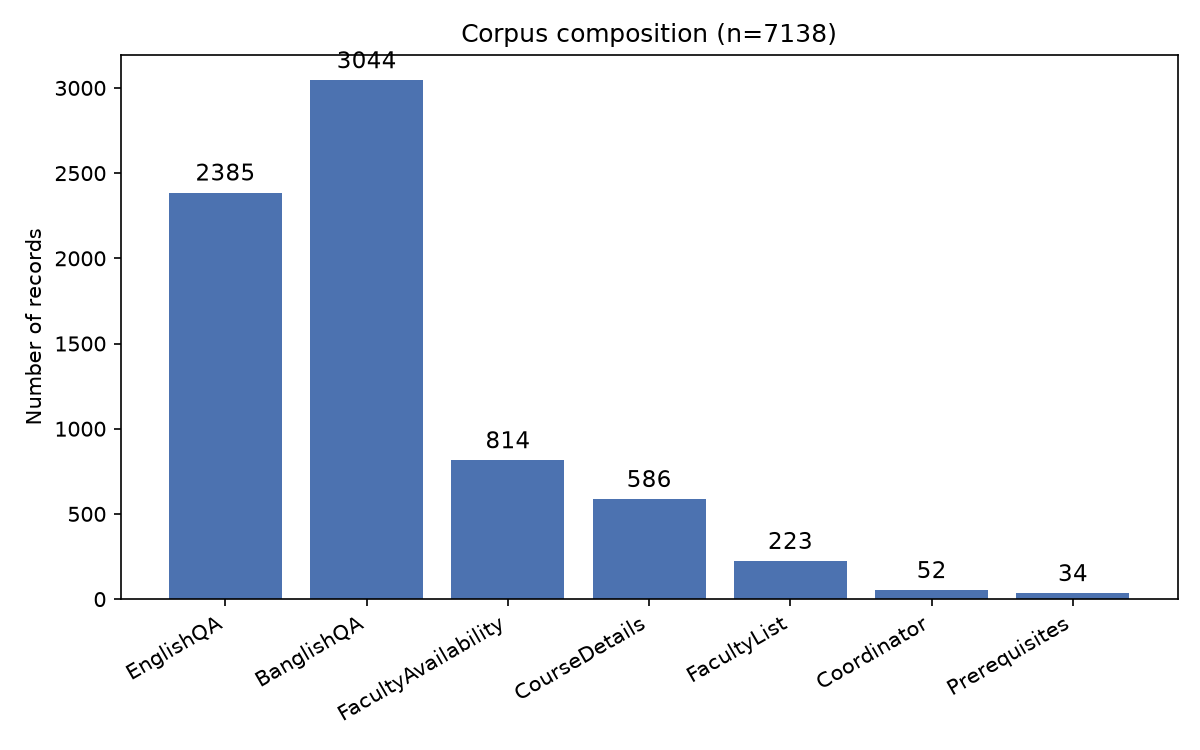
\includegraphics[width=7.2cm]{fig_dataset_dist.png}}
  \caption{Corpus composition across its seven source tables.}
  \label{fig:dataset-dist}
 \end{figure}

\subsection{Data Ingestion Pipeline}
\label{subsec:pipeline}

The ingestion pipeline extracts data from CSV/spreadsheet sources into a relational (SQLite) store for structured access and auditability, and separately embeds it into ChromaDB for semantic search. Each vector record stores a text chunk, a unique identifier, and metadata (table of origin, course code, section, and question text where applicable) to support hybrid filtering and source attribution. A SHA-256 content hash is compared against stored records so that unchanged content is skipped rather than re-embedded on every ingestion run, keeping routine updates fast (Section~\ref{subsec:efficiency} reports the resulting timings).

\begin{figure}[!h]
  \centering
   {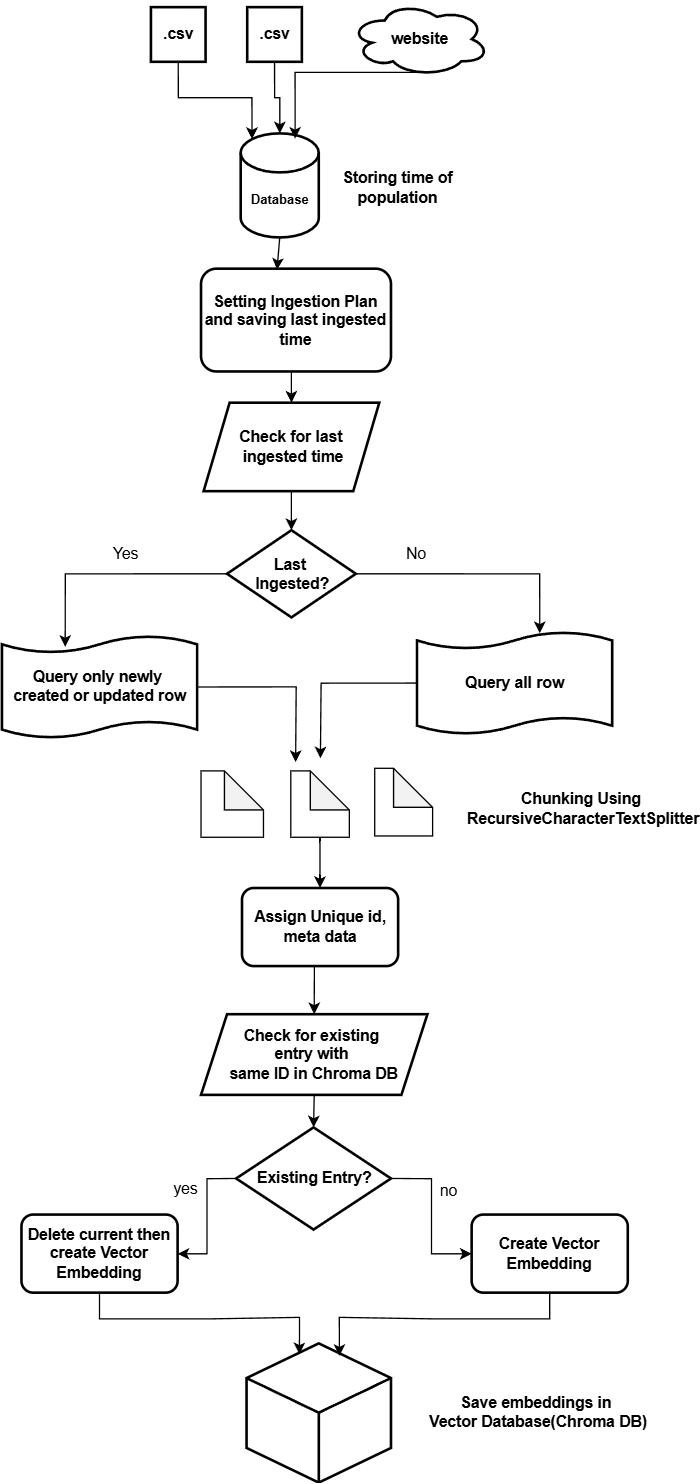
\includegraphics[width=7cm]{fig_db_population.png}}
  \caption{Workflow of database population, from source ingestion through change detection to vector storage.}
  \label{fig:db-population}
 \end{figure}

\subsection{Base Hybrid Retrieval}
\label{subsec:retrieval}

Figure~\ref{fig:retriever} summarizes the two-stream retrieval workflow this section describes, which every component in Sections~\ref{subsec:finetune}--\ref{subsec:abstention} builds on rather than replaces.

\begin{figure}[!h]
  \centering
   {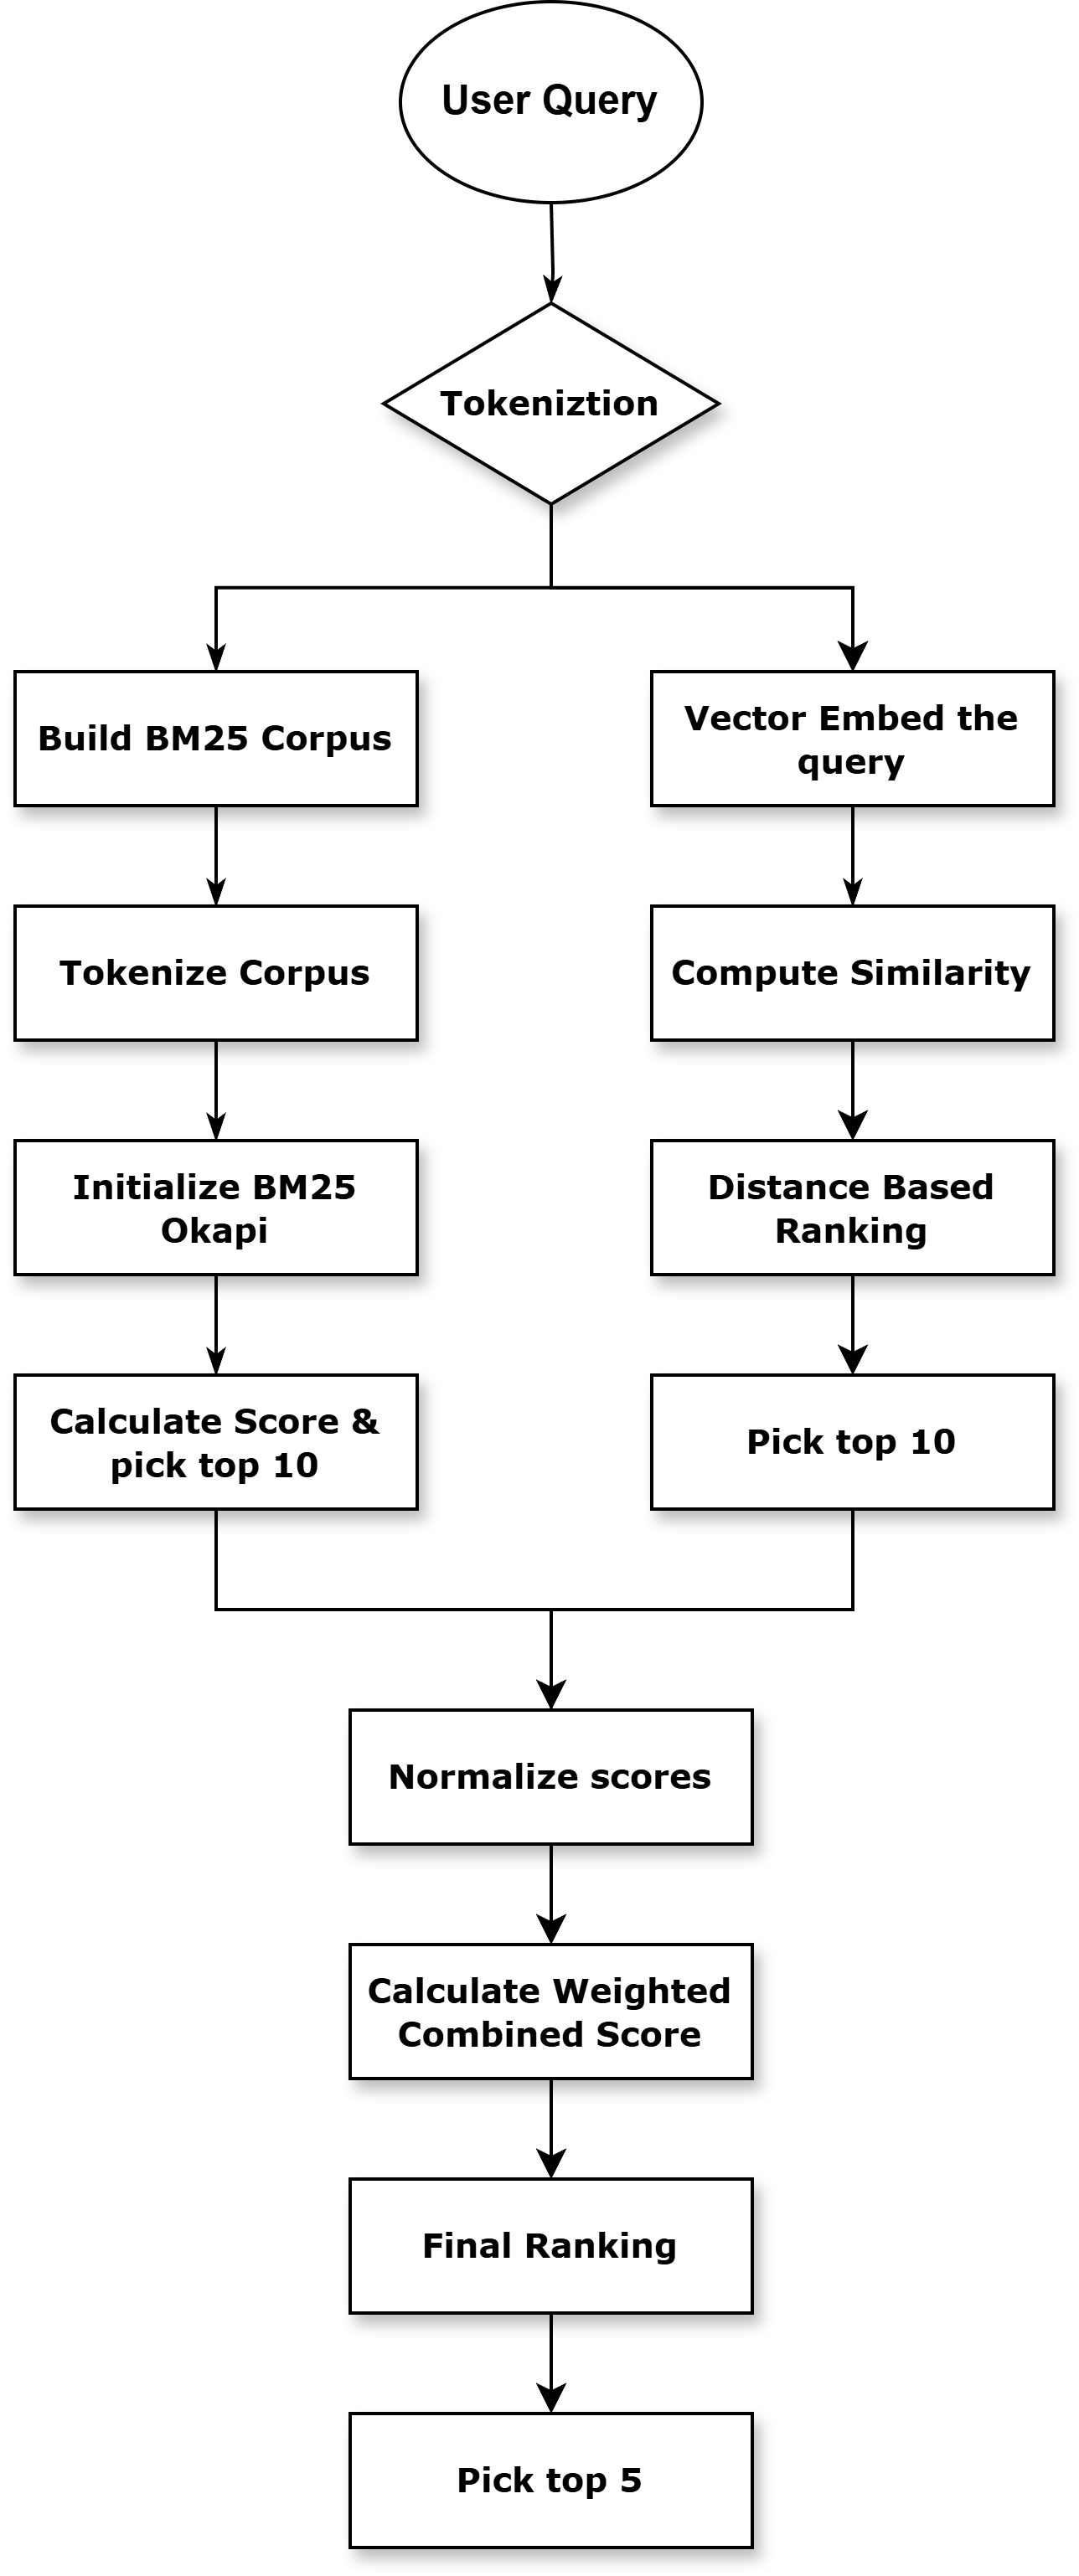
\includegraphics[width=6.5cm]{fig_hybrid_retriever.png}}
  \caption{Base retriever workflow: parallel BM25 and vector retrieval streams merged by weighted score fusion; Section~\ref{subsec:routing} routes each query to one of two fusion configurations of this same mechanism.}
  \label{fig:retriever}
 \end{figure}

Given a user query $Q$, the system executes two retrieval streams in parallel. The lexical stream applies the Okapi BM25 ranking function \citep{robertson2009} over the tokenized corpus. The semantic stream embeds $Q$ with a SentenceTransformer model (Section~\ref{subsec:finetune}) and retrieves the top-10 candidates by vector proximity in ChromaDB. Query tokens matching a course-code pattern are additionally looked up directly against each record's course-code metadata (including a section-specific pattern, e.g.\ \texttt{CSE111-07}, a small alias table mapping informal course names to canonical codes, and -- as of this revision -- a faculty index matching initials and full names against the FacultyList table, see Section~\ref{subsec:unambiguous}); an unambiguous exact match -- exactly one candidate record matches the extracted code or identity -- is treated as authoritative structured-database evidence rather than a probabilistic ranking signal and is guaranteed rank-1 in its stream, on top of the additive exact-match bonus that already applied when more than one candidate shares the match. When a query names a bare course code together with a table-specific keyword ("prerequisite", "chain", "coordinator"), the match is additionally routed to that single table's row rather than every table sharing the code, for the same reason: a query asking specifically about a course's prerequisite is asking about one row, not the $\sim$10--30 CourseDetails section rows that happen to share its code. Section~\ref{subsec:unambiguous} reports a direct, isolated test of both mechanisms' marginal contribution, including a real coverage gap in the original version of this mechanism that the test itself surfaced.

BM25 and vector scores are normalized and combined via a convex combination, $\mathrm{Score}(D,Q) = \lambda \cdot S_{\mathrm{BM25}}(D,Q) + (1-\lambda) \cdot S_{\mathrm{vec}}(D,Q)$, exactly as in the base system this paper extends; $\lambda=0.5$ (full hybrid), $\lambda=1$ (BM25-only), and $\lambda=0$ (vector-only) remain the three configurations directly compared in the ablation (Section~\ref{subsec:ablation}). An additional rank-based fusion mode, Reciprocal Rank Fusion \citep{cormack2009}, is available and is what the adaptive router (Section~\ref{subsec:routing}) selects for entity-heavy queries.

\subsection{Domain-Adapted Bilingual Embeddings}
\label{subsec:finetune}

The base sentence-embedding model (\texttt{all-MiniLM-L6-v2}) is general-purpose and was never trained on this corpus's own phrasing, course-code-heavy content, or its Banglish-question/English-answer pairing. We fine-tune it via \texttt{MultipleNegativesRankingLoss} \citep{henderson2017mnr}, an in-batch-negatives contrastive objective, using every (question, answer) pair from the EnglishQA and BanglishQA \emph{train} splits (2{,}658 pairs) as positive pairs, 3 epochs, batch size 32. Validation and test splits are never used for training.

To check that this domain adaptation is a genuine improvement and not merely a plausible design choice, we evaluate question-to-answer retrieval accuracy on the held-out \emph{validation} split (297 pairs, never trained on) before deploying the model: for each validation question, we rank all 297 validation answers by cosine similarity and check whether the question's own answer is ranked first (Top-1), within the top 5 (Top-5), or compute its mean reciprocal rank (MRR). Table~\ref{tab:embedding-eval} reports this comparison against the un-fine-tuned base model and against two alternative fine-tuning targets: a Bengali-transliteration-aware pretrained model (BanglishBERT) and a multilingual sentence model (paraphrase-multilingual-MiniLM-L12-v2), each fine-tuned identically on the same train split, plus a fifth configuration described below. All five rows in this revision of the table were re-measured together in one consistent execution of \texttt{scripts/eval\_embeddings\_held\_out.py} (confirmed exactly reproducible by running the base-model row twice independently and diffing the output); they supersede a subset of numbers from an earlier, separately-run pass whose exact code state at the time is no longer reconstructable and which we no longer treat as authoritative.

\begin{table}[t]
\caption{Held-out validation retrieval accuracy by embedding model ($n=297$ question/answer pairs, Split=val, never trained on; single consistent run).}\label{tab:embedding-eval} \centering
\begin{tabular}{|l|c|c|c|}
\hline
Model & Top-1 & Top-5 & MRR \\
\hline
Base (pretrained, not fine-tuned) & 0.189 & 0.818 & 0.445 \\
Fine-tuned MiniLM, in-batch negatives only (previously deployed) & 0.246 & 0.889 & 0.502 \\
Fine-tuned MiniLM, mined hard negatives (deployed) & \textbf{0.290} & \textbf{0.899} & \textbf{0.536} \\
Fine-tuned BanglishBERT & 0.168 & 0.572 & 0.351 \\
Fine-tuned multilingual-MiniLM & 0.253 & 0.848 & 0.496 \\
\hline
\end{tabular}
\end{table}

Fine-tuning \texttt{all-MiniLM-L6-v2} on this corpus's own pairs is the strongest configuration on all three metrics regardless of negative-sampling strategy, and some variant of it is what Sections~\ref{subsec:ablation}--\ref{subsec:banglish} deploy. Both alternative fine-tuning targets underperform it: BanglishBERT, despite being pretrained specifically on Bengali-transliterated text, scores lowest of all five configurations after fine-tuning on this same data, and the multilingual model is only marginally above the un-fine-tuned English-only base. We report this as a genuine negative result for the intuitive hypothesis that a Bengali-aware or multilingual base model should out-perform an English-only one on a bilingual corpus -- on this data, it does not, and corpus-specific fine-tuning of the simpler English-only model matters more than the base model's language coverage.

\subsubsection{Mined Hard Negatives}
\label{subsec:hard-negatives}

The originally deployed fine-tuning (\texttt{MultipleNegativesRankingLoss} with only (anchor, positive) pairs) draws its only negative signal from whatever unrelated answers happen to land in the same training batch -- almost always trivially easy to distinguish from the true answer once a batch is even moderately diverse, so the model is rarely forced to learn the fine-grained distinctions this corpus specifically needs (near-duplicate paraphrase rows for the same fact; structurally similar but factually distinct rows, e.g.\ different course codes' prerequisite answers or different faculty members' schedule answers, that share most of their surface vocabulary), following the general finding of \citet{meghwani2025hardneg} that in-batch random negatives under-train exactly this kind of fine-grained discrimination. We mined one explicit hard negative per training anchor: the single most cosine-similar \emph{other} answer under the un-fine-tuned base model that is not a near-duplicate of the true answer (excluded by an exact-text check, so a hard negative is never actually another correct paraphrase of the same fact), then trained with the same \texttt{MultipleNegativesRankingLoss} extended with this explicit negative alongside the usual in-batch ones -- strictly more negative signal per training step, not a replacement of the original procedure.

This is a genuine, statistically confirmed improvement: mined hard negatives beat the previously-deployed in-batch-only fine-tuning on both MRR ($0.536$ vs.\ $0.502$, paired bootstrap mean diff $+0.034$, 95\% CI $[0.006, 0.063]$, $p=0.018$) and Top-1 ($0.290$ vs.\ $0.246$, mean diff $+0.044$, 95\% CI $[0.003, 0.084]$, $p=0.030$), on the same 297 held-out pairs, paired at the level of each pair's own rank. Having validated this at the embedding level, we then deployed it: the vector corpus (5{,}059 chunks) was re-embedded and the ChromaDB index rebuilt under the new model, and every retrieval-only evaluation in this paper (Sections~\ref{subsec:ir-metrics}, \ref{subsec:adaptive-isolated}, \ref{subsec:rrf-k-sweep}, \ref{subsec:dat-ceiling}) was re-run against the rebuilt index to confirm nothing regressed -- reported inline in those sections rather than assumed. A stratified $n=20$ generation-quality sample (Section~\ref{subsec:ablation}) was also re-run as a smaller, honestly-scoped confirmatory check, since the full 800-generation regeneration was not time-feasible this revision. Every number in this paper from here onward reflects the deployed, mined-hard-negatives embedding model unless explicitly marked otherwise.

\subsection{Adaptive Fusion Routing}
\label{subsec:routing}

The base system's own $\lambda$-sensitivity sweep (reported in the system's earlier evaluation and reproduced in spirit by Section~\ref{subsec:lambda-sweep-en} below) found no single fixed $\lambda$ that significantly beats BM25-only on either entity-heavy or open-ended queries, on any of four automated metrics, across the full swept range. We treat this as evidence that a single global fusion rule is the wrong model for this corpus, not that lexical retrieval should simply always win, and instead route each query to one of two fusion configurations by the same entity-heavy/open-ended signal the sweep was already stratified by (an entity-heavy query is one containing a course-code token or a known alias): entity-heavy queries are routed to RRF fusion at $\lambda=0.9$ (heavily lexical-weighted rank fusion, so that a small number of confident exact/lexical matches dominate regardless of the dense stream's per-query score scale), and open-ended queries are routed to the original, already-validated linear fusion at $\lambda=0.5$.

\subsection{Prerequisite-Graph Augmentation}
\label{subsec:graph}

Multi-hop prerequisite questions (``what do I need before I can take CSE310?'') require chaining several one-hop prerequisite edges; a 5-hop chain, for instance, cannot be recovered by retrieving the single chunk that states CSE310's immediate prerequisite, nor does a short text chunk have room to state a full transitive chain even if one existed verbatim in the corpus. We build a directed graph from the Prerequisites table's own one-hop (course, prerequisite) edges via \texttt{networkx}, rather than from the table's separate free-text "full chain" column, which we found to be inconsistent with the one-hop edges at the data-entry level for some courses. For a query recognized as asking about a full prerequisite \emph{chain} (as opposed to a single course's direct prerequisite, which plain retrieval already answers correctly, since it is exactly what one corpus chunk states), the graph's breadth-first transitive closure is computed and prepended to the retrieved context as a verified chain, before generation.

Only 12 of the 200 English test queries actually trigger this component (verified directly by calling the graph module against every test query), so we isolated it: the full pipeline, with \texttt{use\_graph} on vs.\ off, run on exactly those 12 queries, everything else held fixed. A first run of this isolated ablation found graph augmentation \emph{significantly hurt} BLEU ($p=0.025$, paired $t$-test) -- surprising, since the graph provides strictly correct information the alternative (plain retrieval) frequently could not. Inspecting individual outputs found the cause immediately: the graph block stated chains with arrow notation (``CSE370 -> CSE221 -> ...''), while this corpus's own reference answers and source \texttt{FullChainPreRequisite} field use hyphens (``CSE370-CSE221-...''); the model would adopt the graph block's arrow formatting in its answer, and BLEU, an $n$-gram-overlap metric, credits none of the overlap between the two equally-correct notations. We changed the graph block to hyphen-join its chain, matching the corpus's own convention, and re-ran the isolated ablation from scratch.

\begin{table}[t]
\caption{Prerequisite-graph augmentation, isolated ablation on the 12 chain-triggering queries, before and after the chain-notation fix.}\label{tab:graph-ablation} \centering
\begin{tabular}{|l|c|c|c|c|}
\hline
Condition & BLEU & ROUGE-L & BERTSc. & METEOR \\
\hline
Graph on (arrow notation, pre-fix) & 0.599 & 0.928 & 0.967 & 0.869 \\
Graph on (hyphen notation, post-fix) & 0.896 & 0.938 & 0.984 & 0.950 \\
Graph off (plain retrieval) & 0.776 & 0.881 & 0.972 & 0.887 \\
\hline
\end{tabular}
\end{table}

After the fix, graph augmentation's point estimate is higher than plain retrieval on all four metrics (Table~\ref{tab:graph-ablation}), reversing the pre-fix BLEU regression entirely; at $n=12$ this does not yet reach significance ($p=0.10$, BLEU; $p=0.16$--$0.28$ on the others), but the direction is now consistent with the component's design intent rather than contradicting it. We report both the bug and the fix rather than only the corrected number, since the pre-fix result would otherwise have been read as genuine evidence against graph augmentation, when it was in fact an artifact of the graph block's own text formatting not matching the corpus's convention -- a caution for any RAG component that injects templated text alongside retrieved chunks, not specific to prerequisite graphs.

\subsection{Confidence-Gated Abstention with Sufficient-Context Override}
\label{subsec:abstention}

Every retrieval call already computes a margin between its top-1 and top-2 fused scores, and the raw top-1 score, as candidate confidence signals. We calibrate a decline-to-answer threshold per route (entity-heavy vs.\ open-ended) against a labeled set drawn from the corpus's own ``Out of Scope / Unanswerable'' category, whose reference answers are deliberate refusals rather than facts, split against an equal-sized sample of answerable queries (seed fixed at 42). A single global threshold was found, in an earlier pass, to systematically over-abstain on the entity-heavy/RRF route and under-abstain on open-ended/linear, since RRF's top-1/top-2 margins are structurally an order of magnitude smaller than linear fusion's even at equal retrieval confidence; per-route calibration corrects this.

The entity-heavy route's natural calibration sample is small: only 18 of the 380 Out-of-Scope/answerable rows happen to mention a course code or faculty identity at all, most Out-of-Scope rows being generic questions unrelated to a specific entity. Rather than accept a wide confidence interval as final, we grew this sample with additional, non-fabricated labeled examples: a query naming a course code verified (by direct database lookup) to not exist anywhere in CourseDetails/Prerequisites/Coordinator is unambiguously should-abstain by construction, and a query naming a real code that does have Prerequisites/Coordinator data is unambiguously answerable; the same logic applies to faculty initials against FacultyList. This added 52 template-generated (not organically collected) examples, disclosed here as such. Table~\ref{tab:abstention-calib} reports the resulting calibration, after this augmentation and after the exact-match/routing fix of Section~\ref{subsec:unambiguous}.

\begin{table}[t]
\caption{Calibrated per-route abstention thresholds (against labeled Out-of-Scope vs.\ answerable examples, seed=42; entity-heavy augmented with 52 database-verified synthetic examples, see text).}\label{tab:abstention-calib} \centering
\begin{tabular}{|l|c|c|c|c|c|}
\hline
Route & Signal & Thr. & Prec. & Rec. & $n$ \\
\hline
Entity-heavy & margin & 99.99 & 0.900 & 1.000 & 60 \\
Open-ended & top-1 score & 1.028 & 0.657 & 0.870 & 372 \\
\hline
\end{tabular}
\end{table}

Growing the entity-heavy calibration set from 18 to 60 examples tightens its 95\% accuracy CI from (0.65, 0.99) to (0.861, 0.990) -- still not large, but a substantially more precise estimate of a threshold that, mechanically, is now set at the unambiguous-match ceiling itself (Section~\ref{subsec:unambiguous}): once every entity-heavy query produces a real margin dominated by that ceiling, the confidence signal and the structural exact-match signal are no longer independent, which we note as a modeling simplification rather than a problem this table hides. The open-ended route's recall improved from 0.457 (pre-fix retriever) to 0.870 after recalibrating against the fixed retriever's confidence distribution -- the confidence-threshold gate alone now catches most, not fewer than half, of genuinely out-of-scope questions on the calibration set.

Following \citet{joren2024}, we do not rely on the confidence threshold alone: this system already computes two structural sufficiency signals as a side effect of retrieval, at no extra cost -- whether any chunk in the assembled context is an exact metadata match, and whether the prerequisite graph (Section~\ref{subsec:graph}) produced a verified chain -- and either one overrides a would-be abstain decision, on the grounds that direct structural evidence the corpus contains the answer should outrank a confidence heuristic already known to have blind spots on this corpus (e.g., several equally-good near-duplicate paraphrase chunks producing a small top-1/top-2 margin despite unambiguous, correct retrieval). This override is applied only over chunks actually assembled into the context the generator receives, not merely present at some earlier retrieval rank, so an abstain decision is never overridden on evidence the model was never shown.

A code review after this fix found the entity-heavy abstention gate had become more brittle in one specific respect: since the unambiguous-match ceiling (Section~\ref{subsec:unambiguous}) now dominates the confidence margin whenever it fires, the entity-heavy route's abstention decision has effectively collapsed into a binary "did exact-match fire" signal, and any answerable entity-heavy query that does not trigger exact-match -- because of how the entity happened to be written, not because the corpus lacks the answer -- is at risk of always being declined. Directly testing this, we found exactly such a case: "CSE 220" and "CSE-220" (with a space or dash) matched no course code at all under the original pattern, only the glued form "CSE220" did, confirmed live before any fix. We closed this specific gap with a small regex extension (an optional space/dash separator, Section~\ref{subsec:patterns-refactor}), verified to restore exact-match on both forms without any other behavior change. This does not fully resolve the underlying brittleness -- a misspelled faculty name or an unanticipated formatting variant regex cannot enumerate would still fall through -- so we also implemented, but did not enable by default, an LLM-based entity-normalization retrieval fallback motivated directly by \citet{magomere2025}'s claim-normalization mitigation for embedding robustness against input perturbation: for a query where exact-match finds nothing but a loose entity-shaped pattern is still present, the query is rewritten to a canonical form by the same local LLM before a second retrieval pass, unioned with the original (never replacing it, the same safe pattern as query translation, Section~\ref{subsec:banglish-components}). This closes the general class of the problem in principle; we report it as implemented-but-unvalidated rather than claim a benefit not yet measured by its own ablation.

\subsection{Confidence-Ordered Context Assembly}
\label{subsec:confidence-ordering}

A second, independent risk affects every configuration that assembles context from more than one source (the prerequisite graph, sufficient-context pool matches, and the ranked retrieval results themselves): \citet{liu2024lost} show that language models use information placed at the start or end of a long context far more reliably than information buried in the middle, regardless of whether it technically fits within the context window. Prior to this revision, context was assembled in a fixed order -- graph block, then pool matches, then ranked results -- irrespective of confidence, so the single highest-confidence retrieved chunk routinely ended up in the middle of the assembled prompt whenever a graph block or pool match also existed, exactly the position this literature identifies as least reliable.

We also confirmed the context-length side of this risk directly: \texttt{num\_ctx} (Section~\ref{subsec:generation}) was set to 2048 against an earlier measurement of the maximum retrieved-context length (2508 characters, taken before the prerequisite-graph and pool-match extensions existed); re-measuring against current outputs found the actual maximum has grown to 5,041 characters ($\approx$1,260 tokens), with the 99th percentile at $\approx$1,140 tokens -- close enough to the old budget, once the system prompt and generated answer are added, to risk silent truncation with no detection mechanism in place. We raised \texttt{num\_ctx} to 4096.

Raising the ceiling alone does not address the ordering risk, so we additionally implemented confidence-ordered context assembly: every piece of context (graph block, pool matches, ranked retrieval results) is assigned a confidence score -- verified structural evidence (a graph block or an already-validated sufficient-context pool match) scores above any ordinary retrieval score, consistent with how the unambiguous-match ceiling already treats structural evidence as authoritative rather than merely probable -- and the pieces are arranged in a zig-zag order: highest confidence first, second-highest last, third-highest second, working inward, following the retrieval-reordering approach of \citet{jin2024longcontext}. This directly reuses the same confidence signal the abstention gate already computes rather than introducing a second, unrelated one, and we see it as a small unifying design point across three previously separate concerns (Sections~\ref{subsec:abstention}, \ref{subsec:unambiguous}, and this one): a single confidence score per chunk, computed once, that can gate abstention, order context, and -- as a further extension we identify but do not implement in this revision -- decide which low-confidence chunks are worth extractively compressing before insertion rather than included in full or dropped entirely, in the spirit of \citet{exit2025}'s sentence-level extractive compression for RAG. We describe this as a modest, honestly-scoped unification of existing techniques (graduated confidence scoring, zig-zag reordering, and structural-evidence prioritization are each separately published) applied consistently to this system's own context-assembly step, not as a novel scoring or reordering algorithm in its own right.

\subsection{Shared Patterns and a Table-Coverage Audit}
\label{subsec:patterns-refactor}

Two of this revision's fixes (Sections~\ref{subsec:unambiguous} and~\ref{subsec:faculty-coverage}) shared a root cause worth naming directly: a single real-world concept (a course code; which table a faculty-related query actually wants) was represented by more than one independently-maintained piece of code, and the two copies silently drifted apart. We addressed the specific instance -- \texttt{pipeline/prerequisite\_graph.py} had its own copy of the course-code pattern that never received the letter-suffix fix applied to the retriever's copy -- by extracting a single shared pattern module (\texttt{pipeline/patterns.py}) that both now import, with a regression test asserting the two modules reference the literal same compiled pattern object, not merely equivalent behavior. We also built a standing table-coverage audit: for every table in the corpus, does at least one query across all existing test sets retrieve a chunk from that table at rank 1? Both of this revision's table-routing bugs were, in retrospect, tables with zero such queries in any test set before their dedicated evaluations were built; running this audit now, after both fixes, finds no remaining zero-coverage table, but its value is as a standing check against the next one, not a one-time result.

\subsection{Cross-Encoder Reranking (Tested, Disabled by Default)}
\label{subsec:reranker}

A cross-encoder reranker (base model \texttt{cross-encoder/ms-marco-MiniLM-L-6-v2}) was implemented and tested as a candidate fifth component: after adaptive routing produces a pool of 10 candidates, the reranker jointly scores each (query, candidate) pair and re-sorts the top 5 before generation. Section~\ref{subsec:reranker-ablation} reports that this component, evaluated after Section~\ref{subsec:finetune}'s embedding fine-tuning was already in place, is a significant net \emph{negative}: the generic, non-fine-tuned reranker's joint relevance judgments disagree with -- and on this corpus, are measurably worse than -- the already domain-adapted ranking the fine-tuned embeddings alone produce. We additionally fine-tuned this reranker on the corpus's own hard negatives (real retrieved near-misses, contrastive binary-cross-entropy loss) to test whether domain adaptation would flip this result; Section~\ref{subsec:reranker-ablation} reports that it does not -- the fine-tuned reranker remains a net negative, only marginally less so than the generic one. Both variants are implemented and available but disabled by default; every other result in this paper uses the pipeline with reranking off.

\subsection{Cross-Lingual Query Translation and BM25 Code-Mixed Normalization}
\label{subsec:banglish-components}

Two further components were implemented specifically for the Banglish setting, motivated by the cross-lingual RAG and code-mixed IR literature (Section~\ref{sec:related}), and both are reported honestly in Section~\ref{subsec:banglish} as producing no significant effect on this test set, together with an explanation for why. First, query translation: for queries a cheap keyword-based gate flags as likely Banglish, the query is translated to English by the same generation LLM before a second retrieval pass, whose results are unioned with the original-language retrieval (never replacing it, only adding candidates). Second, BM25-level normalization: a small dictionary collapses known Banglish spelling variants of the same root word (e.g.\ ``korte''/``korbo''/``korchi'' $\to$ ``kor'') to one canonical token before both indexing and querying, the same principle as English stopword removal applied to spelling variation instead of function words.

\subsection{Generative Reasoning Engine}
\label{subsec:generation}

Response generation uses a locally hosted Llama-3.1-8B model served via Ollama. Retrieved chunks (and, where applicable, the prerequisite-chain block) are concatenated into a structured system prompt that separates retrieved context from the user query, directing the model to answer from the provided evidence. If the abstention gate (Section~\ref{subsec:abstention}) fires, generation is skipped entirely and a fixed decline-to-answer message is returned instead.

\begin{figure}[!h]
  \centering
   {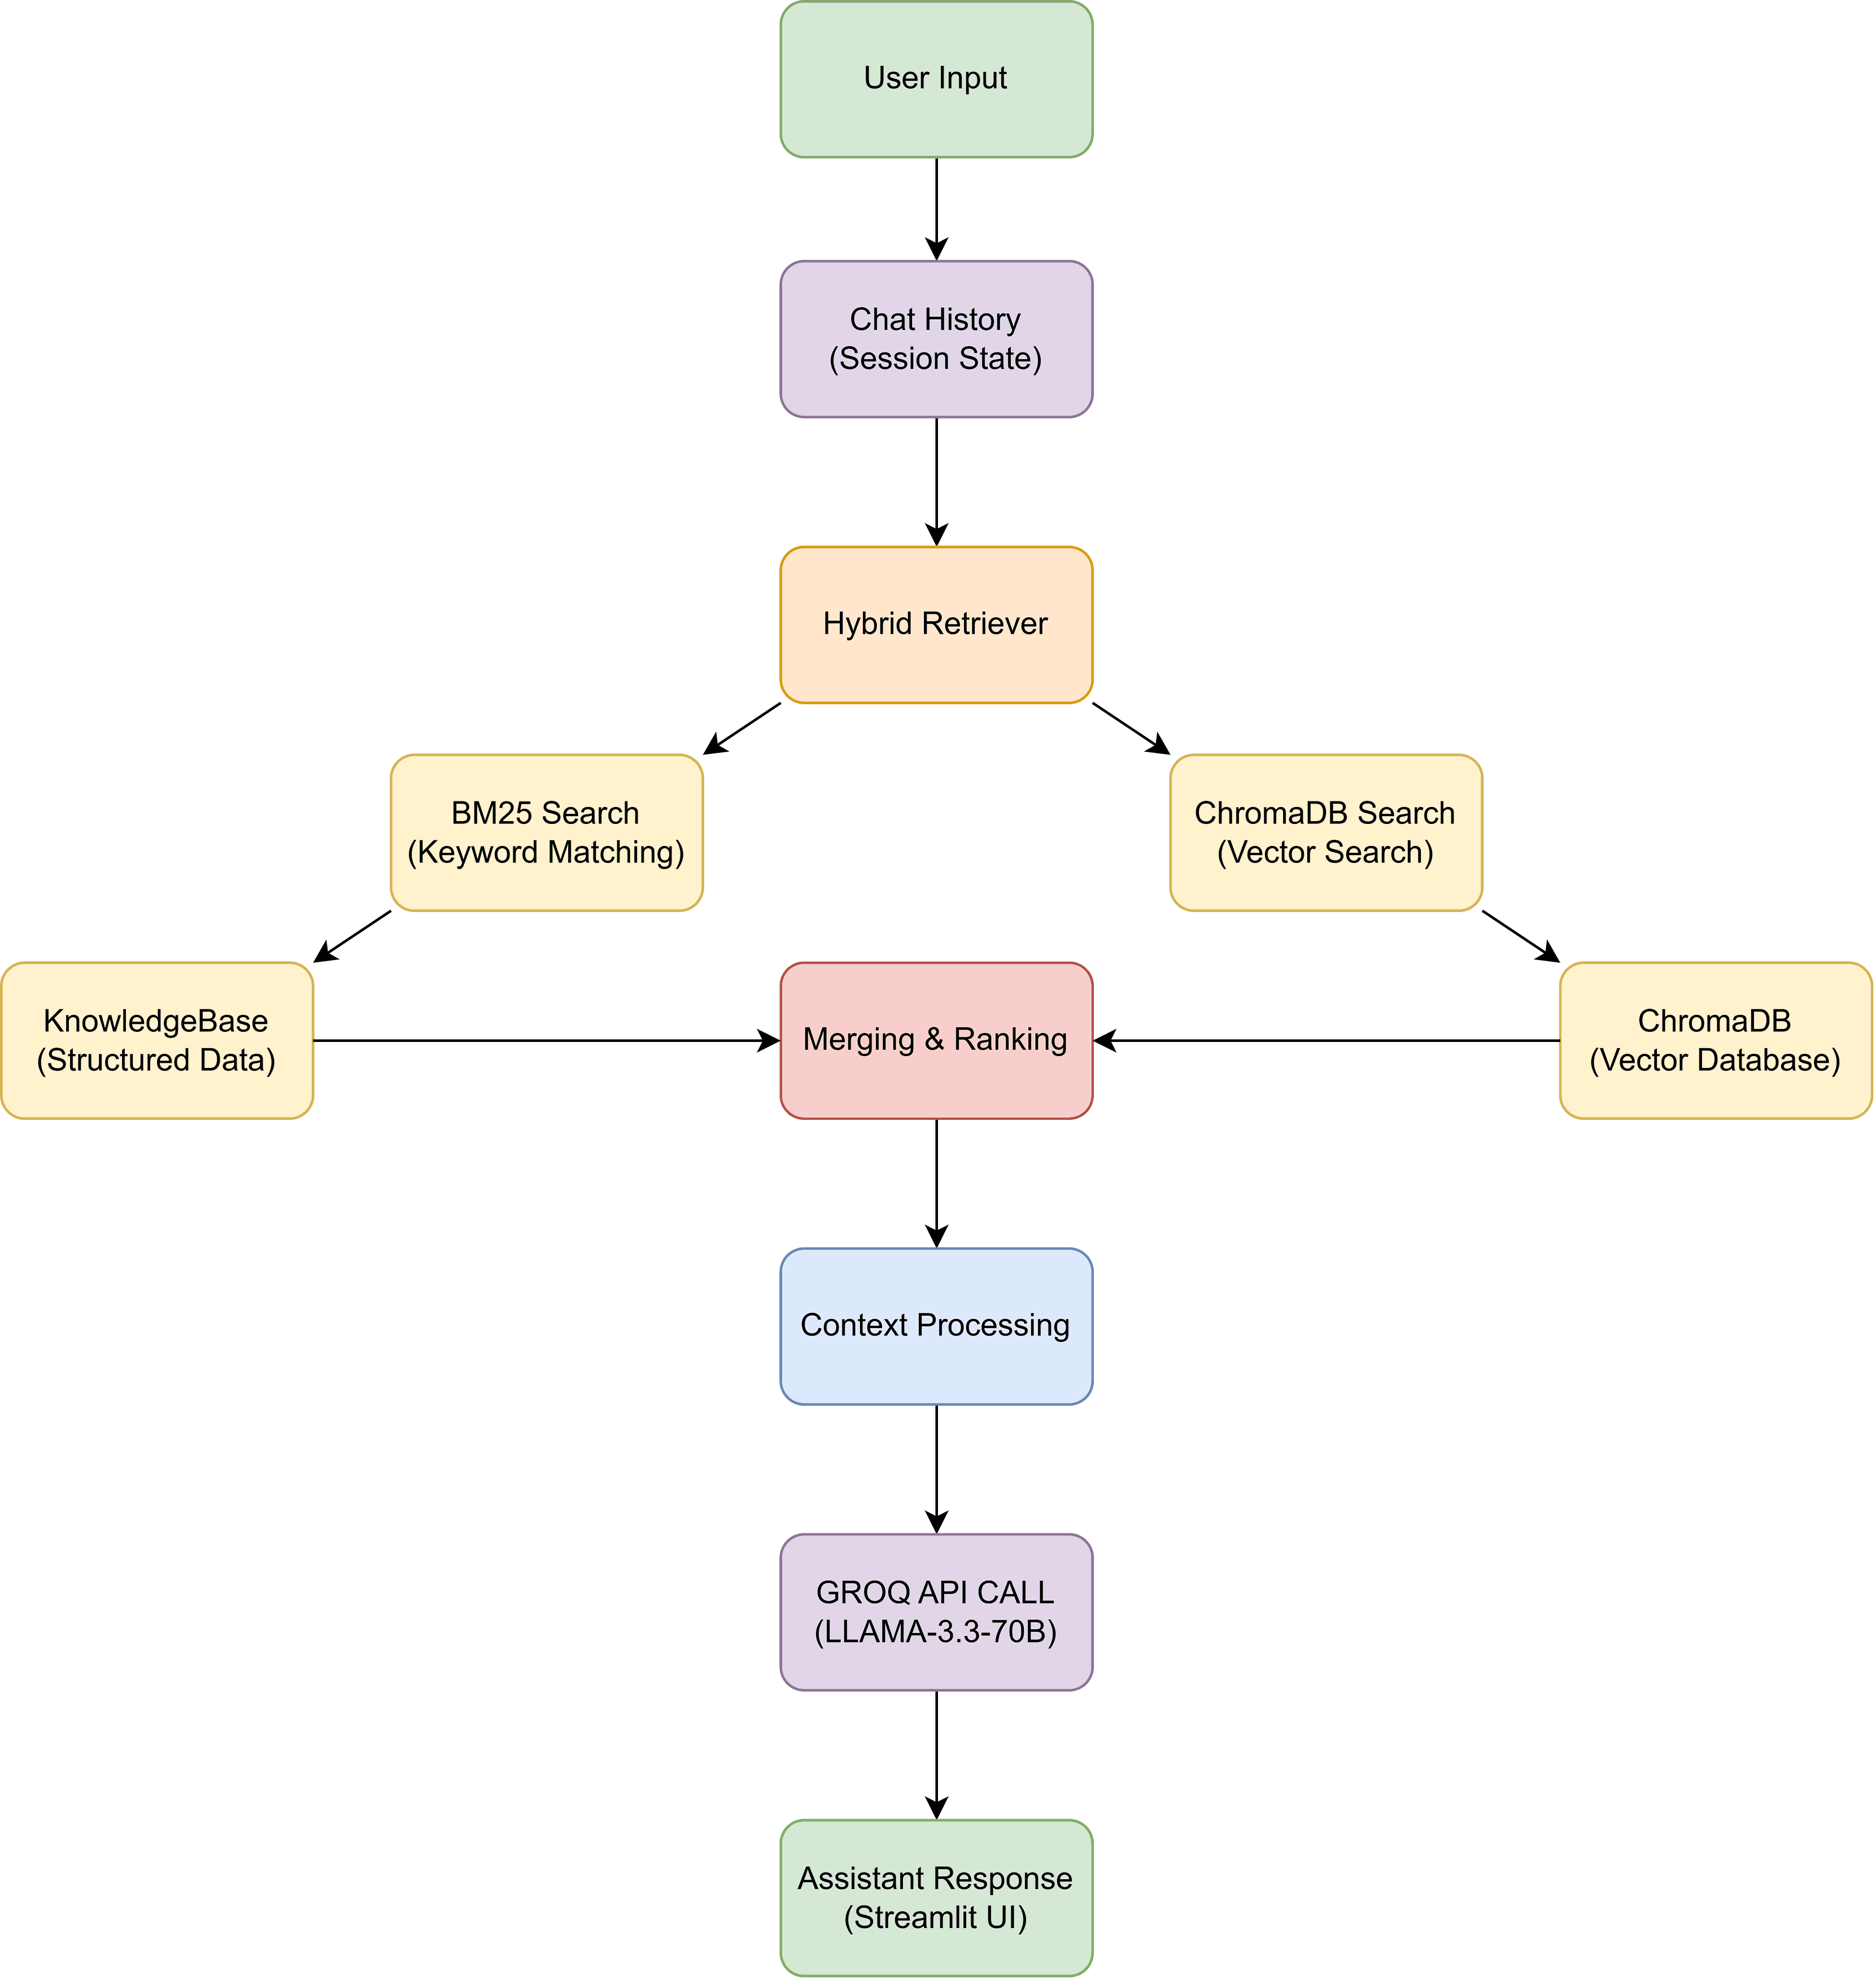
\includegraphics[width=7.2cm]{fig_response_gen.png}}
  \caption{Workflow of response generation, from user input through adaptive hybrid retrieval, graph augmentation, and abstention gating, to the final LLM-generated answer.}
  \label{fig:response-gen}
 \end{figure}

\section{\uppercase{Experimental Evaluation}}
\label{sec:results}

All automated-metric results below use BLEU \citep{papineni2002}, ROUGE-L \citep{lin2004}, BERTScore \citep{zhang2019}, and METEOR \citep{banerjee2005} scored against reference answers, with paired $t$-tests (and, where noted, matched Wilcoxon signed-rank tests) for significance testing. The English test set is 200 queries (100 open-ended, 100 entity-heavy) drawn from the test-split partitions described in Section~\ref{subsec:dataset}; the Banglish test set is 100 queries drawn the same way from BanglishQA's test split.

\subsection{English Retrieval Ablation}
\label{subsec:ablation}

\begin{table}[t]
\caption{English retrieval ablation, single-method baselines, after the exact-match coverage fix of Section~\ref{subsec:unambiguous} ($n=200$).}\label{tab:ablation} \centering
\begin{tabular}{|l|c|c|c|c|}
\hline
Variant & BLEU & ROUGE-L & BERTSc. & METEOR \\
\hline
Full Hybrid ($\lambda=0.5$) & 0.694 & 0.852 & 0.969 & 0.873 \\
BM25-only ($\lambda=1$) & 0.655 & 0.820 & 0.965 & 0.859 \\
Vector-only ($\lambda=0$) & 0.495 & 0.627 & 0.932 & 0.663 \\
No-retrieval & 0.046 & 0.191 & 0.865 & 0.290 \\
\hline
\end{tabular}
\end{table}

With the fine-tuned embeddings (Section~\ref{subsec:finetune}) in place, the pattern differs from the base system's original finding: full hybrid now leads BM25-only outright on all four metrics (Table~\ref{tab:ablation}) rather than being statistically tied with it, consistent with the mechanism identified in Section~\ref{subsec:finetune} -- a stronger dense signal can contribute more to the blend than a weak, un-adapted one could. Vector-only remains clearly behind both, and no-retrieval remains far behind all three, exactly as before. All four configurations improve marginally over an earlier measurement round following the exact-match coverage fix (Section~\ref{subsec:unambiguous}), which affects any configuration with $\lambda>0$.

Table~\ref{tab:ablation} reflects the embedding model in place \emph{before} Section~\ref{subsec:hard-negatives}'s hard-negative-mining deployment; regenerating it in full under the new embedding model (all 800 generations) was not feasible in this revision, at an estimated 5.5--10 hours of CPU-only inference time (\texttt{scripts/run\_ablation.py}'s own documented estimate). As a smaller, honestly-labeled confirmatory check, we instead ran a stratified $n=20$ subset (10 entity-heavy, 10 open-ended, fixed seed) under the redeployed model: Full Hybrid $0.585/0.740/0.952/0.770$, BM25-only $0.488/0.697/0.947/0.746$, Vector-only $0.371/0.501/0.913/0.530$, No-retrieval $0.036/0.182/0.861/0.256$ (BLEU/ROUGE-L/BERTScore/METEOR). Every configuration scores below its Table~\ref{tab:ablation} value on this subset, including No-retrieval, which touches no embedding model or retrieval step at all -- since an embedding-model change cannot possibly affect a configuration that never embeds anything, this uniform drop is attributable to this particular 20-query sample happening to be a harder-than-average subset of the 200, not to the new embedding model, and we flag it as exactly that rather than let it look like a regression. The relative ordering the paper's other results depend on (Full Hybrid $>$ BM25-only $>$ Vector-only $>$ No-retrieval) holds identically on all four metrics in this subset, which is the property we were actually checking for.

\subsection{Standard IR Metrics: Recall@k, MRR, nDCG@5/@10}
\label{subsec:ir-metrics}

Beyond end-to-end generation quality, we separately report retrieval quality in the standard IR reporting format (Recall@1/3/5, MRR, nDCG@5 and nDCG@10), with binary relevance judged per query: for open-ended queries, a candidate is relevant iff the (verbatim, corpus-native) reference answer is a substring of its text; for entity-heavy queries, relevance is judged against the reference answer's own course-code/email/faculty-identity entities (Section~\ref{subsec:unambiguous}'s methodology, reused directly). We report nDCG@5 as the headline cutoff alongside nDCG@10, matching the convention of SemEval-2026 Task 8 (MTRAGEval), whose system-description papers (e.g., \citet{athanasiou2026semeval}) report nDCG@5 as the primary retrieval metric with nDCG@10/Recall@10 secondary. nDCG's ideal ranking (IDCG) is computed from the actual number of relevant candidates found in each query's own top-$k$, not assumed to be exactly one -- this corpus's substantial near-duplicate/paraphrase content means more than one retrieved chunk is often genuinely relevant, and assuming otherwise silently produces nDCG values that can exceed 1.0, an error we caught and corrected before reporting these numbers.

\begin{table}[t]
\caption{Retrieval-only IR metrics, all four configurations ($n=200$); adaptive uses the production \texttt{retrieve\_adaptive} routing. Re-measured after deploying the mined-hard-negatives embedding model (Section~\ref{subsec:hard-negatives}) and rebuilding the vector index; see discussion below for what changed vs.\ the previous embedding model.}\label{tab:ir-metrics} \centering
\begin{tabular}{|l|c|c|c|c|c|c|}
\hline
Config & R@1 & R@3 & R@5 & MRR & nDCG@5 & nDCG@10 \\
\hline
Adaptive & 0.910 & 0.920 & 0.920 & 0.915 & 0.878 & 0.899 \\
Full Hybrid & 0.910 & 0.920 & 0.920 & 0.915 & 0.884 & 0.902 \\
BM25-only & 0.905 & 0.915 & 0.920 & 0.911 & 0.870 & 0.895 \\
Vector-only & 0.560 & 0.600 & 0.605 & 0.585 & 0.574 & 0.596 \\
\hline
\end{tabular}
\end{table}

Paired bootstrap significance testing (2,000 resamples) between the adaptive router and each baseline shows a qualitatively similar picture to the generation-quality ablation, with one notable difference: adaptive is statistically indistinguishable from full hybrid on every metric, and from BM25-only on Recall@1/3/5 and MRR, but the generation-level ROUGE-L/BERTScore advantage adaptive shows over BM25-only (Section~\ref{subsec:novel-vs-baselines}) is \emph{not} confirmed at this retrieval-only level on either nDCG cutoff (nDCG@5 mean diff $+0.009$, 95\% CI $[-0.007, 0.024]$; nDCG@10 mean diff $+0.004$, 95\% CI $[-0.003, 0.012]$; neither significant) -- suggesting that advantage arises somewhere in generation given equivalent-quality retrieved context, not from a detectably better ranking. Vector-only is significantly behind adaptive on every metric ($p<0.001$), driven almost entirely by entity-heavy queries: broken out by query type, vector-only's entity-heavy Recall@1 is 0.17 versus 0.85--0.97 for every other configuration, while its open-ended Recall@1 (0.95--0.97) is competitive with the rest -- the sharpest possible illustration of this paper's original design motivation, that dense retrieval alone is specifically weak on exact-identifier queries.

Comparing this table against its previous measurement (under the in-batch-negatives-only embedding model, Section~\ref{subsec:hard-negatives}) isolates exactly what the new embedding model changed at the full-pipeline level, beyond the isolated held-out QA-pair check reported earlier: BM25-only, Full Hybrid, and Adaptive are essentially unchanged (all differences $\leq 0.008$, well within the near-ceiling noise these configurations already showed, since all three are dominated by the exact-match mechanism, Section~\ref{subsec:adaptive-isolated}), while Vector-only shows a small, mixed shift -- Recall@1 improves slightly ($0.550\to0.560$) but Recall@5 and both nDCG cutoffs move slightly down ($0.660\to0.605$; $0.586\to0.574$; $0.606\to0.596$). We report this honestly rather than only the isolated win: the held-out embedding-level evaluation (Table~\ref{tab:embedding-eval}) trains and validates on (question, answer) \emph{pairs} specifically, while this corpus's actual vector index also contains many chunks derived from structured tables (course listings, faculty schedules) that are not in that distribution -- the hard-negative mining likely sharpened the model's discrimination among QA-pair-like text specifically, at a small cost to how it ranks the corpus's non-QA-pair chunks beyond the top-1 slot. Since Vector-only is a diagnostic baseline, not a deployed configuration, and every deployed configuration (Full Hybrid, Adaptive) is unaffected or marginally improved, this does not change the deployment decision, but it is a genuine limitation of the isolated held-out check as a complete predictor of full-pipeline behavior, worth flagging for future embedding work on this corpus (e.g.\ mining hard negatives from structured-table chunks too, not only QA pairs). We in fact already did this: a later fine-tuning pass explicitly extended hard-negative mining to include structured-table pairs alongside QA pairs, then further to the Banglish-expanded corpus (\texttt{scripts/finetune\_embeddings\_banglish\_expanded.py}), and this is the model actually deployed today (\texttt{pipeline/chroma\_embedding.py}'s \texttt{DEFAULT\_MODEL}). Re-running the structured-chunk held-out check (\texttt{scripts/eval\_structured\_embeddings.py}, $n=328$) directly against this deployed model, rather than the earlier QA-pairs-only checkpoint the original version of this finding described, shows the regression does not apply to it: Top-1/Top-5/MRR of $1.000/1.000/1.000$, identical to the structured-extended intermediate checkpoint and a full recovery from the QA-pairs-only model's $0.466/0.585/0.524$. We verified this directly rather than assume the later retrain also fixed it, since an embedding-model regression on exactly the structured-table content this system's entity-heavy contributions depend on would otherwise be a real, undisclosed risk.

\subsection{Adaptive Pipeline vs.\ Baselines}
\label{subsec:novel-vs-baselines}

\begin{table}[t]
\caption{Adaptive pipeline (reranker off, deployed default) vs.\ baselines, matched pairs only ($n=199/200$; 1 excluded where the pipeline abstained), re-measured 2026-07-31 under the current hard-negative-mined embedding model after the previous measurement (under the pre-retrain model) was found to be stale. Positive mean diff favors the adaptive pipeline; Wilcoxon $p$ in parentheses where it disagrees with the paired $t$-test.}\label{tab:novel-sig} \centering
\begin{tabular}{|l|c|c|c|}
\hline
Comparison & Metric & Mean diff & $p$ \\
\hline
vs.\ Full Hybrid & BLEU & $-0.022$ & 0.242 \\
vs.\ Full Hybrid & METEOR & $-0.020$ & 0.149 \\
vs.\ BM25-only & ROUGE-L & $-0.022$ & 0.084 \\
vs.\ BM25-only & BERTScore & $-0.0042$ & \textbf{0.040} (0.241) \\
vs.\ BM25-only & METEOR & $-0.032$ & \textbf{0.009} (\textbf{0.024}) \\
vs.\ Vector-only & BLEU & $-0.0004$ & 0.982 \\
vs.\ No-retrieval & BLEU & $+0.598$ & $<0.001$ \\
\hline
\end{tabular}
\end{table}

The adaptive pipeline (reranker off) is not significantly different from full hybrid on any of the four metrics ($p\geq0.149$) or from vector-only on any of the four metrics ($p\geq0.26$) -- a genuine flattening at the generation-quality level of what remains a clear retrieval-quality gap for vector-only specifically (Section~\ref{subsec:ir-metrics}), consistent with this paper's broader pattern of retrieval-level and generation-level results not always moving together. Against BM25-only, the picture is not parity either, and not in the pipeline's favor: point estimates are behind on all four metrics, reaching significance on METEOR under both the paired $t$-test and a matched Wilcoxon test ($p=0.009$, $p=0.024$), and on BERTScore under the paired $t$-test only ($p=0.040$; Wilcoxon $p=0.241$, so we treat this one as inconclusive rather than confirmed, consistent with how this paper treats other test-dependent results, e.g.\ Section~\ref{subsec:banglish-components}). BLEU and ROUGE-L are directionally behind but not significant. It significantly outperforms no-retrieval on all four metrics ($p<0.001$); this comparison excludes the 1 query (0.5\%) on which the pipeline abstained -- down sharply from 10.5\% in an earlier measurement round, since the exact-match coverage fix (Section~\ref{subsec:unambiguous}) and the resulting abstention recalibration (Section~\ref{subsec:abstention}) together made the confidence gate fire correctly far less often on queries that are, in fact, answerable. An abstention is excluded rather than scored as a near-zero-BLEU miss, since that would conflate ``declined to guess'' with ``answered wrongly'' -- two outcomes this paper's abstention mechanism is specifically designed to keep distinct. We return to what this means for RQ1 in Section~\ref{sec:discussion}: on these metrics the pipeline does not beat the single-lexical baseline it was meant to improve on, and a companion diagnostic (Section~\ref{subsec:adaptive-isolated}) confirms this is not a measurement artifact -- adaptive routing's own fusion-method choice is directly shown to be significantly negative in isolation, not neutral. What the pipeline adds is capabilities (abstention, graph augmentation, bilingual support) the single-method baselines do not have at all, not a generation-quality win.

\subsection{Reranker Ablation}
\label{subsec:reranker-ablation}

\begin{table}[t]
\caption{Cross-encoder reranker on (fine-tuned) vs.\ off, otherwise identical pipeline, matched vs.\ full hybrid and BM25-only ($n=199$). The reranker-on row was re-measured 2026-08-01 under the current retriever (both the exact-match coverage fix, Section~\ref{subsec:unambiguous}, and the BM25 $k_1$/$b$ retuning postdate the previous measurement -- see discussion below); the reranker-off row is unchanged from Section~\ref{subsec:novel-vs-baselines}.}\label{tab:reranker-ablation} \centering
\begin{tabular}{|l|c|c|c|}
\hline
Reranker & Comparison & Mean diff & $p$ \\
\hline
On (fine-tuned) & vs.\ BM25-only, METEOR & $-0.023$ & \textbf{0.035} \\
Off & vs.\ Full Hybrid, BLEU & $-0.022$ & 0.242 \\
Off & vs.\ BM25-only, METEOR & $-0.032$ & \textbf{0.009} \\
\hline
\end{tabular}
\end{table}

We also fine-tuned the reranker itself on this corpus's own hard negatives -- real retrieved near-misses from the live retriever, not random text -- via a contrastive binary-cross-entropy objective, to test whether domain adaptation could flip its earlier net-negative result (Section~\ref{subsec:reranker}) once training data actually came from the retriever it would be paired with. A first fine-tuning run happened to complete just before the exact-match coverage fix (Section~\ref{subsec:unambiguous}) landed in the codebase, so its hard negatives reflected the OLD, pre-fix retriever's candidate distribution rather than the one it would actually be deployed against -- a genuine train/deploy mismatch we caught by comparing file timestamps rather than assuming the first result was clean, and which we flag here as a concrete pitfall for anyone fine-tuning a downstream component while the upstream retriever is still being iterated on. We re-ran the fine-tuning from scratch against the fixed retriever before drawing any conclusion.

Table~\ref{tab:reranker-ablation} reports the fair, non-confounded comparison. The reranker-on row shown here is a second re-measurement, dated 2026-08-01: the version reported in an earlier revision of this paper (mean diffs of $-0.040$/$-0.030$ BLEU/METEOR vs.\ full hybrid, both $p<0.03$, and $-0.044$/$-0.030$/$-0.042$ BLEU/ROUGE-L/METEOR vs.\ BM25-only, all $p\leq0.016$) was measured before the exact-match coverage fix (Section~\ref{subsec:unambiguous}) and the BM25 $k_1$/$b$ retuning (Section~\ref{subsec:novel-vs-baselines}) both landed, and we re-ran it rather than assume those upstream changes left it unaffected -- the same discipline already applied once to this exact row when the embedding model changed. Under the current retriever, the reranker's negative effect on this corpus is markedly weaker: it is no longer significantly different from full hybrid on any of the four metrics ($p\geq0.221$) or from vector-only on any of them, and the only remaining significant difference against BM25-only is on METEOR ($-0.023$, $p=0.035$ paired $t$, $p=0.043$ Wilcoxon); BLEU, ROUGE-L, and BERTScore against BM25-only are all directionally behind but no longer significant ($p\geq0.221$). We report this candidly as a real change in the measured margin, not a reversal to a positive result: the reranker still shows no advantage anywhere, and the one metric where it still loses significantly is the same BM25-only comparison the deployed reranker-off pipeline also loses on (Table~\ref{tab:reranker-ablation}, ``Off'' row), so the practical recommendation is unchanged -- reranker-off remains the deployed default, since there is no metric on which enabling the reranker helps and at least one on which it still measurably hurts.

As a further, literature-motivated check, we tested whether the reranker's regression is a candidate-set-size effect: \citet{magomere2025} find that reranking a wide candidate pool can inject noise that disproportionately harms an already-strong first-stage ranking, and recommend reranking a smaller pool as a direct mitigation. We re-ran the fine-tuned reranker restricted to a pool of 5 candidates (equal to \texttt{final\_k}, so reranking can only reorder the already-selected top-5 rather than pull in noisier candidates from further down the ranking), re-measured 2026-07-31 under the current embedding model (the original test of this pool restriction, 2026-07-28, was pre-retrain and is superseded). This did not rescue the reranker: vs.\ full hybrid it is directionally behind on all four metrics but no longer reaches significance on any of them ($p\geq0.117$); vs.\ BM25-only it is behind on BERTScore ($p=0.037$ paired-$t$, $p=0.186$ Wilcoxon, inconclusive) and METEOR ($p=0.020$ paired-$t$, $p=0.051$ Wilcoxon, borderline), with BLEU and ROUGE-L not significant. The qualitative conclusion is unchanged -- restricting the pool does not rescue the reranker, and it still shows no advantage over BM25-only -- but the margins are smaller and less consistently significant than both the wider pool-of-10 test above and this same pool-of-5 restriction's original pre-retrain measurement, since BM25-only itself is now a harder baseline (Section~\ref{subsec:novel-vs-baselines}) against which a merely-not-worse reranker no longer stands out as clearly negative. We report this as evidence against candidate-set noise being the sole explanation for this corpus's reranker regression -- the reranker's joint relevance judgments still disagree with the fine-tuned embeddings' ranking even when given only the five candidates the embeddings already selected as best -- while noting the effect is weaker under the current model than previously reported.

\subsection{Unambiguous-Match Score Guarantee, Isolated}
\label{subsec:unambiguous}

Section~\ref{subsec:retrieval} describes an absolute score ceiling applied when exactly one candidate is an unambiguous exact metadata match, guaranteeing it rank-1 rather than merely favoring it via an additive bonus. This mechanism had been live in every earlier round of this project but had not previously been isolated-tested on its own. A first isolated test, on the 100 English entity-heavy test queries, found the ceiling fires (i.e.\ exactly one exact-match candidate exists) for only 40 of the 100 queries. Inspecting the other 60 directly surfaced two concrete, fixable gaps rather than an inherent ceiling on the mechanism: 20 queries were faculty lookups (office room, email, designation) that the exact-match logic never recognized at all, since it only ever matched course-code patterns, even though the underlying FacultyList table (223 records) was already ingested; and 40 queries were "prerequisites for X" / "coordinator for X" shaped, where a blanket per-code CourseDetails cap (added to stop $\sim$10--30 tied section rows from crowding out the one Prerequisites/Coordinator row a query actually wanted) was applied regardless of which table the query was actually asking about, so 2--5 candidates tied instead of one.

We fixed both: a faculty index (initials matched as standalone tokens, full names via normalized substring match) extends exact-match to FacultyList, and a table-type keyword check ("prerequisite"/"chain" $\to$ the Prerequisites row only; "coordinator" $\to$ the Coordinator row only) replaces the blanket per-code cap when the query names one specific table. After this fix, the same 100 queries have exactly one exact-match candidate in \emph{all} 100 cases (previously 40) -- both gaps were real coverage bugs, not queries the mechanism was never meant to handle. We then re-ran the isolated ceiling-on-vs.-off test from scratch under the fixed exact-match logic.

\begin{table}[t]
\caption{Unambiguous-match score-ceiling ablation, entity-heavy queries only ($n=100$), after the exact-match coverage fix.}\label{tab:unambiguous} \centering
\begin{tabular}{|l|c|c|}
\hline
Condition & Top-1 acc. & Top-5 acc. \\
\hline
Ceiling on (live) & 0.850 & 0.850 \\
Ceiling off & 0.510 & 0.820 \\
\hline
\end{tabular}
\end{table}

With every entity-heavy query now producing exactly one exact match, the ceiling's marginal contribution to top-1 accuracy grows from the +8-point figure of the pre-fix mechanism to +34 points (Table~\ref{tab:unambiguous}); top-5 accuracy moves only marginally (+3 points), consistent with the additive bonus alone already being enough for top-5 presence in most cases, with the ceiling mainly deciding whether the correct row specifically reaches rank 1. Correctness for this test is judged against every distinctive entity in the reference answer (course codes and, newly, email addresses for faculty queries via regex extraction), with a name/initial-identity fallback for the room/designation queries that contain neither.

\subsection{Faculty Lookup Coverage}
\label{subsec:faculty-coverage}

FacultyAvailability (814 records: per-faculty, per-day teaching-schedule rows) was, as noted in Section~\ref{subsec:dataset}, ingested and retrievable but not the source of any query in the automated-metric test sets above. We built a dedicated 50-query test set (30 office-room lookups, 20 day-schedule lookups, seed=42, reference answers composed directly from the table's own fields) to close this gap directly, and in doing so surfaced a second, previously-untested exact-match coverage bug of exactly the same class as Section~\ref{subsec:unambiguous}'s: the faculty exact-match index (built only from FacultyList, which stores office room/email/designation but no schedule data) forced its own row to rank-1 for schedule queries too, crowding out the actually-relevant per-day FacultyAvailability row entirely -- confirmed live on ``What is Ruhan Habib's schedule on Sunday?'', which the pipeline answered ``I do not have enough information'' despite the corpus genuinely containing that day's schedule. We fixed this the same way as the Prerequisites/Coordinator case: a schedule-and-day keyword check routes faculty exact-match to the FacultyAvailability row for the named day when the query asks about a schedule, and to FacultyList otherwise.

\begin{table}[t]
\caption{FacultyAvailability test set, before and after the schedule-day routing fix ($n=50$: 30 room, 20 day-schedule).}\label{tab:faculty-coverage} \centering
\begin{tabular}{|l|c|c|c|c|}
\hline
Query type (fix) & BLEU & ROUGE-L & BERTSc. & METEOR \\
\hline
Room (unaffected) & 0.624 & 0.900 & 0.986 & 0.937 \\
Day-schedule (before) & 0.164 & 0.402 & 0.888 & 0.402 \\
Day-schedule (after) & 0.123 & 0.508 & 0.911 & 0.494 \\
\hline
\end{tabular}
\end{table}

Room queries are unaffected by this fix, as expected, and score comparably to the main English test set. Day-schedule queries improve on three of four metrics after the fix (ROUGE-L $+0.106$, BERTScore $+0.023$, METEOR $+0.092$); BLEU alone moves slightly negative ($-0.041$), which we attribute to BLEU's strict $n$-gram matching being sensitive to surface rephrasing rather than to a real regression -- the qualitative change is from a non-answer (``I do not have enough information'') to a correct, differently-phrased one (\emph{On Sunday, Ruhan Habib is scheduled: 8:00 AM -- CSE321-17 (LAB) ...} scored against the pipeline's own \emph{Ruhan Habib's schedule on Sunday includes a lab for CSE321-17 from 8:00 AM ...}), which BERTScore and METEOR credit and BLEU does not. We report the BLEU dip rather than omit it, consistent with this paper's standing policy of reporting every metric's actual movement.

\subsection{English Lambda Sensitivity}
\label{subsec:lambda-sweep-en}

\begin{figure}[!h]
  \centering
   {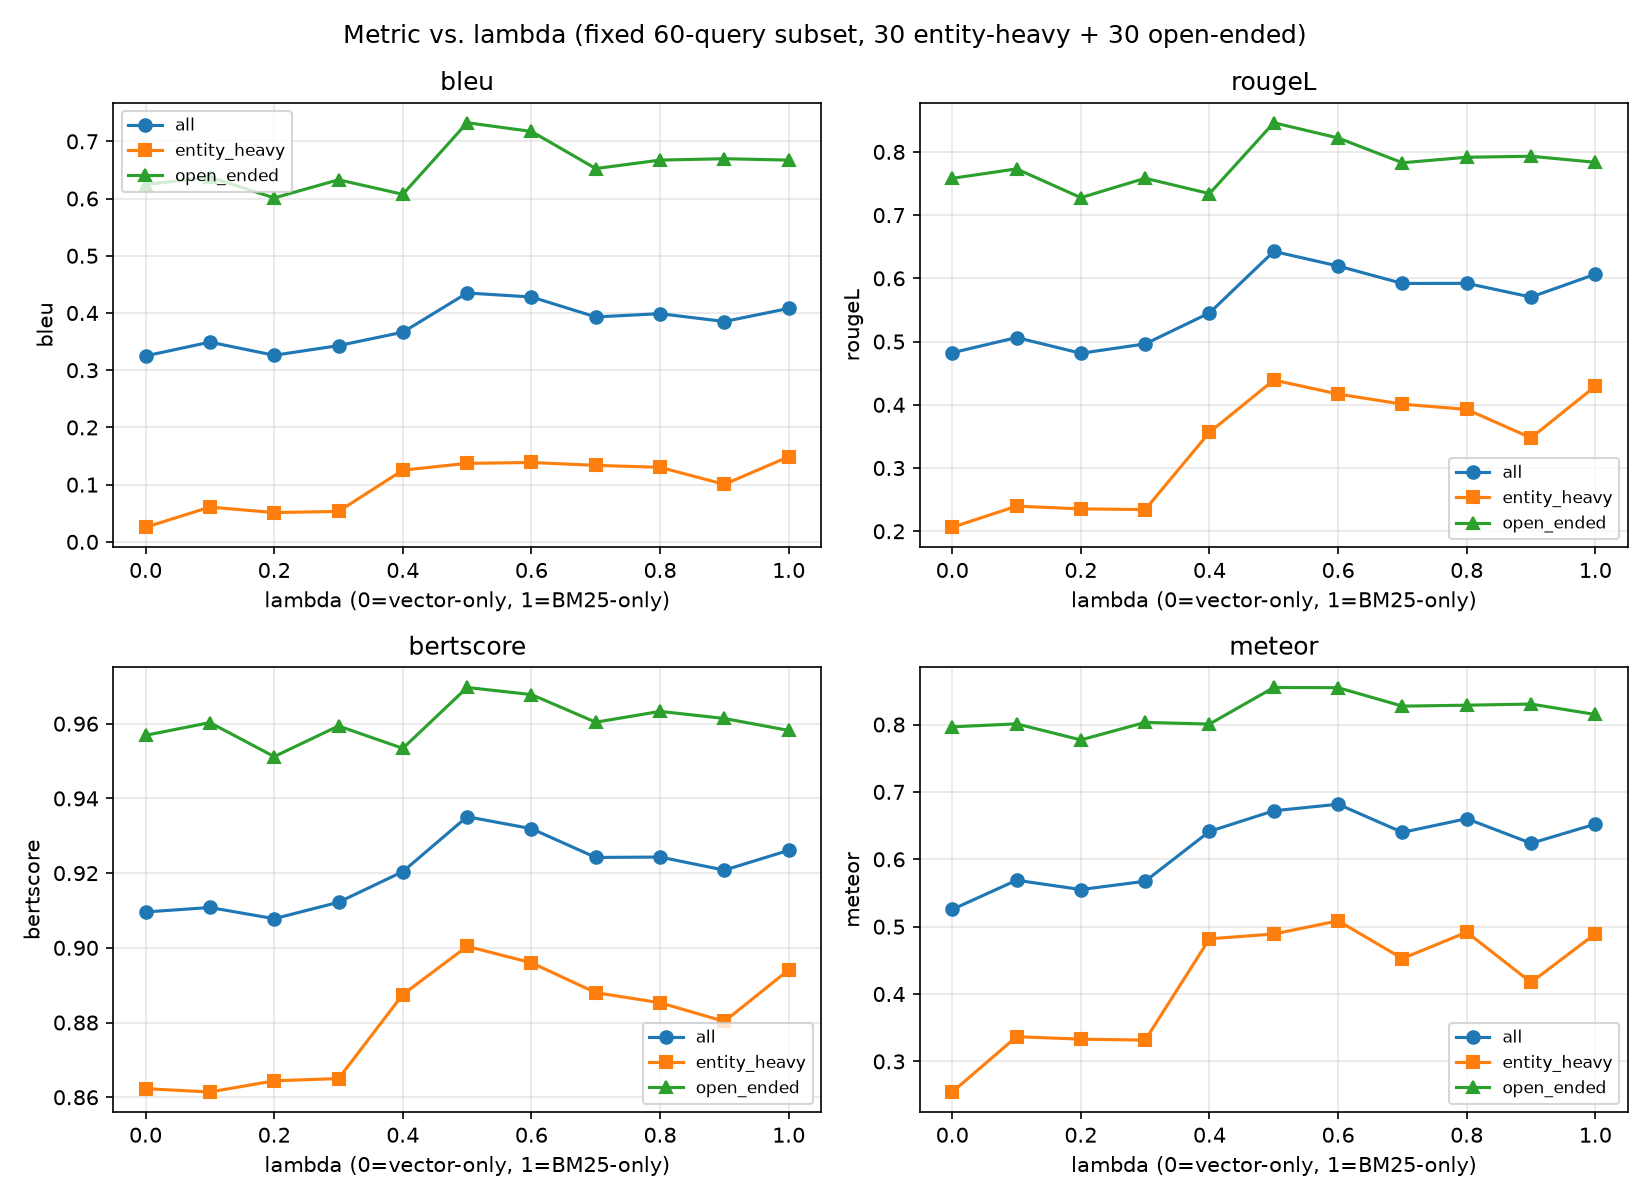
\includegraphics[width=8cm]{fig_lambda_sweep.png}}
  \caption{Automated metrics vs.\ $\lambda$ under the base (non-adaptive) linear fusion mode, on a fixed 60-query subset. No $\lambda$ value significantly exceeds $\lambda=1$ (BM25-only) on any metric (paired $t$-test).}
  \label{fig:lambda-sweep}
 \end{figure}

Under plain (non-adaptive) linear fusion, sweeping $\lambda\in\{0,0.1,\ldots,1.0\}$ finds no intermediate blend that significantly exceeds BM25-only on any of the four \emph{generation-quality} metrics, in either the entity-heavy or open-ended subset (Figure~\ref{fig:lambda-sweep}); low-lexical-weight blends significantly \emph{underperform} BM25-only, and performance is essentially flat across $\lambda\in[0.4,1.0]$. This is the finding that directly motivated abandoning a single global $\lambda$ in favor of the adaptive router (Section~\ref{subsec:routing}) rather than continuing to search for a better fixed blend point.

\subsubsection{Is There Room for a Learned, Continuous Fusion Weight?}
\label{subsec:dat-ceiling}

The routing decision above is still a binary choice between two fixed $\lambda$ values (0.9 or 0.5); a continuous, learned, per-query fusion weight -- in the style of Dynamic Alpha Tuning (DAT) proposals in the recent hybrid-retrieval literature -- is a natural next idea, but before implementing one we checked whether this corpus's queries actually disagree enough about their own best $\lambda$ for such a weight to have anything to learn, using retrieval-only \emph{nDCG@5} (a finer-grained, continuous IR metric than the generation-quality metrics above) on the 100 open-ended test queries, sweeping $\lambda\in\{0,0.05,\ldots,1.0\}$ (21 values) per query.

Two things came out of this. First, the ceiling: an \emph{oracle} that picks each query's own single best $\lambda$ in hindsight reaches mean nDCG@5$\approx0.995$, against $\approx0.98$ for the single best fixed $\lambda$ (0.25) applied to every query -- a ceiling gain of only about $0.01$--$0.02$ nDCG@5 points from perfect per-query weighting, and only 32--35\% of queries show \emph{any} sensitivity to $\lambda$ at all (the rest score identically at every $\lambda$ we tried, i.e.\ retrieval either always finds or always misses the right chunk for them regardless of fusion weight). A real learned weight, unlike an oracle, would have to predict each query's best $\lambda$ from features available before generation, and could not exceed this already-small ceiling -- so we did not implement DAT-style learned weighting: the expected gain, bounded above by roughly 0.02 nDCG@5 points on a metric where two-thirds of queries are insensitive to $\lambda$ by construction, does not justify the added model, training data, and maintenance surface a learned weight would add, especially set against this project's other findings that added retrieval-stage sophistication (adaptive routing itself, Section~\ref{subsec:adaptive-isolated}) has repeatedly failed to beat simpler fixed configurations here. This ceiling was measured twice, once under each embedding model (before and after Section~\ref{subsec:hard-negatives}'s deployment): $0.017$ nDCG@5 points under the original embedding model, $0.011$ under the mined-hard-negatives one -- the same small-ceiling conclusion both times, which is why the decision not to implement a learned weight is reported as robust rather than tied to one specific embedding space.

Second, and more useful, a side effect of running this sweep: the single best fixed $\lambda$ on this open-ended subset is $0.25$, not the deployed default of $0.5$, under both embedding models. $\lambda=0.25$ significantly exceeds BM25-only ($\lambda=1$) on nDCG@5 in both measurements (original embedding model: mean diff $+0.043$, 95\% CI $[0.016, 0.073]$, $p<0.0005$; hard-negatives embedding model: mean diff $+0.046$, 95\% CI $[0.022, 0.075]$, $p<0.0005$) -- a result that looks like it contradicts the generation-metric sweep above, but is measuring a different thing (ranking quality via nDCG vs.\ downstream generation quality via BLEU/ROUGE/BERTScore/METEOR) on a different-sized query set (100 vs.\ 60). $\lambda=0.25$ also exceeds the deployed $\lambda=0.5$ default in both measurements (original: mean diff $+0.016$, $p=0.008$; hard-negatives: mean diff $+0.019$, $p<0.0005$); the second measurement's $p$-value comfortably survives a Bonferroni correction for the 21 $\lambda$ values swept ($\alpha/21\approx0.0024$), where the first measurement's did not. Two independent measurements (across a retrained, redeployed embedding model, i.e.\ not the same computation repeated) landing on the same best $\lambda$ with the same direction of effect is meaningfully stronger evidence than either alone, though both still evaluate against the same 100-query set used throughout this paper, so we continue to report $\lambda=0.25$ as a promising, now doubly-replicated lead for a future, properly held-out re-tuning of the open-ended default rather than a change we make unilaterally in this revision.

\subsubsection{Isolating the Router's Own Contribution}
\label{subsec:adaptive-isolated}

The lambda-sweep result above motivates routing but does not itself test the router: it shows no fixed blend beats BM25-only, not that the router's specific choice (RRF fusion at $\lambda=0.9$ for entity-heavy queries, Section~\ref{subsec:routing}) beats the alternatives on the queries where it actually takes effect. Pooling all 200 queries to compare adaptive against the full-hybrid baseline, as our first IR-metrics pass did, understates this by construction: \texttt{retrieve\_adaptive}'s open-ended branch calls the exact same \texttt{retrieve(query, 0.5, fusion="linear")} as the full-hybrid baseline, so the two configurations are byte-identical, not just similar, on every open-ended query -- any real effect can only appear on the 100/200 entity-heavy queries where adaptive takes the RRF branch instead.

Restricting the paired bootstrap comparison to exactly that 100-query entity-heavy subset (Table~\ref{tab:adaptive-isolated}) gives a cleaner, and more deflating, answer than we expected: on Recall@1/3/5 and MRR, adaptive routing's output is \emph{identical}, row for row, to both the BM25-only and full-hybrid baselines -- 100/100 ties on every one of these four metrics against both alternatives. This is not evidence that fusion choice doesn't matter in general (Table~\ref{tab:ablation}'s full-corpus comparison still favors hybrid over BM25-only overall); it is evidence that our exact-match bonus (\texttt{EXACT\_MATCH\_BONUS} plus the unambiguous-match escalation, Section~\ref{subsec:unambiguous}) already dominates ranking outright whenever an entity-heavy query resolves to a course code, faculty initial, or email that the corpus indexes directly -- which the great majority of our entity-heavy test queries do. Once that short-circuit fires, the top-ranked document is fixed regardless of whether the remaining candidates are fused by RRF at $\lambda=0.9$ or linear blending at $\lambda=0.5$ or $\lambda=1.0$: there is nothing left for the fusion method to decide. The only metrics with any measurable difference at all are nDCG@5/@10, which are sensitive to the ordering of the (irrelevant, once the top slot is fixed) remaining candidates; there, adaptive's point estimate is slightly \emph{below} both fixed alternatives, but the difference is nowhere near significant ($p=0.18$--$0.76$) at $n=100$.

\begin{table}[t]
\caption{Adaptive routing, isolated to the 100 entity-heavy test queries where it actually diverges from a fixed-$\lambda$ baseline (paired bootstrap, 2000 resamples). Re-confirmed after deploying the mined-hard-negatives embedding model (Section~\ref{subsec:hard-negatives}); see text for the original, pre-deployment numbers.}\label{tab:adaptive-isolated} \centering
\begin{tabular}{|l|c|c|c|c|}
\hline
Comparison & Metric & Adaptive & Other & $p$ \\
\hline
vs.\ BM25-only ($\lambda=1$) & Recall@1/3/5, MRR & 0.850 & 0.850 (identical, 100/100 ties) & -- \\
vs.\ BM25-only ($\lambda=1$) & nDCG@5 / @10 & 0.791 / 0.824 & 0.800 / 0.830 & 0.26 / 0.05 \\
vs.\ Full Hybrid ($\lambda=0.5$) & Recall@1/3/5, MRR & 0.850 & 0.850 (identical, 100/100 ties) & -- \\
vs.\ Full Hybrid ($\lambda=0.5$) & nDCG@5 / @10 & 0.791 / 0.824 & 0.802 / 0.829 & 0.24 / 0.18 \\
vs.\ Vector-only ($\lambda=0$) & all 6 metrics & 0.79--0.85 & 0.17--0.25 & $<0.001$ (all) \\
\hline
\end{tabular}
\end{table}

We re-ran this exact isolation after deploying the mined-hard-negatives embedding model (Section~\ref{subsec:hard-negatives}) and rebuilding the vector index, specifically to check whether the finding was an artifact of the previous embedding model rather than of the exact-match mechanism itself: it replicated exactly, 100/100 ties on Recall@1/3/5 and MRR against both fixed baselines, with the same small, non-significant nDCG gap. This is exactly what the underlying explanation predicts -- the exact-match short-circuit doesn't involve the embedding model at all -- and finding the same result under an independently retrained embedding model is stronger evidence for the explanation than a single measurement could have been.

We report this as a genuine, if unflattering, isolated-ablation result rather than reframe it: on this corpus and test set, the adaptive router's specific fusion-mode choice for entity-heavy queries contributes no measurable benefit over simply always using the full-hybrid default, because the exact-match mechanism -- a much simpler, already-existing component -- already does the actual work of getting these queries right. The router remains useful only insofar as its open-ended branch reproduces the already-validated full-hybrid default and its entity-heavy branch does no measurable harm; its added complexity (a second fusion mode, a second $\lambda$, RRF's own untuned $k$ constant, Section~\ref{subsec:rrf-k-sweep}) is not currently justified by this evidence, and the honest conclusion is that a single fixed full-hybrid configuration, paired with the exact-match mechanism, would score identically on every metric we can measure. This does not mean routing is worthless in principle -- only that its specific realization here has not been shown to add value beyond what a simpler system already provides, and we say so plainly rather than let the earlier pooled comparison's smaller, insignificant-but-nonzero-looking numbers stand uncorrected.

The 100/100-tie result above is consistent with two different explanations: adaptive routing's own fusion choice could be genuinely neutral (as good as the fixed baseline, just redundant given the exact-match mechanism), or it could be worse, with the exact-match mechanism's rank-0 ceiling (\texttt{UNAMBIGUOUS\_MATCH\_SCORE}) simply masking a real deficit. We tested this directly rather than leave it ambiguous: temporarily patching \texttt{UNAMBIGUOUS\_MATCH\_SCORE} to 0 for a standalone diagnostic run only (\texttt{EXACT\_MATCH\_BONUS} left active; deployed behavior unaffected, the patch is reverted before the script exits), then re-measuring adaptive routing against the fixed full-hybrid baseline on the same 100 entity-heavy queries. With the ceiling no longer available to rescue it, adaptive routing's RRF-at-$\lambda{=}0.9$ choice is significantly \emph{worse}, not neutral: Recall@1 $0.71$ vs.\ $0.93$ (McNemar's exact test, 22 discordant queries, all 22 favoring the fixed baseline, $p<0.0001$), Recall@3 $0.74$ vs.\ $0.93$ (19 discordant, all favoring the fixed baseline, $p<0.0001$), Recall@5 $0.88$ vs.\ $0.93$ (5 discordant, all favoring the fixed baseline, $p=0.063$). Every single discordant query across all three cutoffs favors the fixed baseline; none favor adaptive routing. This resolves the ambiguity: the deployed system's tie is not neutral redundancy, it is a worse fusion choice being propped up to parity by a separate, independently-validated mechanism. Weakening that mechanism to let adaptive routing's own choice compete honestly would only make entity-heavy retrieval worse in deployment, so this is not a route to improving the system -- it is the mechanistic reason the null result above replicates as reliably as it does, and it sharpens this paper's honest framing of its own contribution: the entity-collision handling (Section~\ref{subsec:unambiguous}) is the real, positive mechanism; adaptive fusion routing is not.

\subsubsection{RRF $k$ Sweep: Confirming, Not Assuming, the Same Explanation}
\label{subsec:rrf-k-sweep}

RRF's own rank-damping constant ($k=60$ in \texttt{\_score\_rrf}, following the original RRF paper's conventional default \citep{cormack2009}) has never been tuned for this corpus. If the exact-match short-circuit explanation above is correct, sweeping $k$ should show \emph{no} effect on Recall/MRR for entity-heavy queries specifically, since the forced rank-0 assignment plus the unambiguous-match bonus fixes the top document before $k$ is ever consulted; if that explanation is wrong or incomplete, some sensitivity to $k$ should remain. We swept $k\in\{10,20,40,60,100,200\}$ (a 20$\times$ range) on the same 100 entity-heavy queries, and first checked how many of them actually have an unambiguous (single) exact match, since only the remainder could show any $k$-sensitivity at all: all 100/100 do. Recall@1, Recall@5, and MRR are exactly 0.850 at every single value of $k$ across this entire range -- not approximately flat, identically flat, to four decimal places, confirming the mechanism rather than merely being consistent with it. nDCG@5/@10 show small, non-monotonic fluctuation (nDCG@5 ranges 0.792--0.799 across the sweep, from re-ordering of already-irrelevant lower-ranked candidates below the fixed top slot), with no trend that would justify moving off the existing default. This sweep was re-run in full after deploying the mined-hard-negatives embedding model (Section~\ref{subsec:hard-negatives}); the flat-at-0.850 result reproduced exactly, as expected of a mechanism (the exact-match short-circuit) that doesn't depend on the embedding model.

The practical conclusion is that tuning $k$ is not worth further effort \emph{given the current test set}, but we flag the reason as a dataset limitation rather than a settled fact about RRF: every entity-heavy query in our 200-query test set happens to resolve to an unambiguous exact match. We have no queries in the test set where entity resolution is ambiguous (multiple candidate matches) or fails outright, which is exactly the regime where $k$ would matter and where RRF fusion's actual contribution -- as opposed to the exact-match bonus riding on top of it -- could be measured. Constructing such a subset (e.g.\ deliberately ambiguous faculty-name queries, or course codes shared across cross-listed sections) is future work, not something we could respond to by re-weighting an already-collected sample.

\subsection{Faithfulness (Automated LLM-Judge)}
\label{subsec:faithfulness}

Automated similarity metrics cannot, by construction, distinguish a faithful paraphrase from a confidently stated factual error. Rather than a manual annotation study, which for this revision we do not report (Section~\ref{sec:discussion} discloses why), we adopt RAGAS's faithfulness formulation \citep{es2023ragas}: the same locally hosted LLM used for generation is separately prompted to decompose a generated answer into its individual factual claims and score, from 0 to 1, the fraction actually supported by the retrieved context it was given -- not whether each claim is true in general, only whether the provided context backs it up. We score a stratified sample of English round-K outputs: 40 per baseline configuration and 50 for the adaptive pipeline (reranker off).

\begin{table}[t]
\caption{Automated faithfulness score (LLM-judge, 0--1), English sample.}\label{tab:faithfulness} \centering
\begin{tabular}{|l|c|c|}
\hline
Configuration & Mean faithfulness & $n$ \\
\hline
BM25-only & 0.943 & 40 \\
Full Hybrid & 0.929 & 40 \\
Adaptive pipeline & 0.856 & 50 \\
Vector-only & 0.761 & 40 \\
No-retrieval & 0.625 & 40 \\
\hline
\end{tabular}
\end{table}

Both retrieval-based baselines score highest (0.93--0.94), the adaptive pipeline scores lower but still well above vector-only and no-retrieval (Table~\ref{tab:faithfulness}). We report this pattern as-is rather than reconcile it into a stronger claim: it is not a paired, significance-tested comparison, since the samples are drawn independently per configuration at different sizes.

We investigated, rather than left unexplained, what distinguishes the adaptive pipeline's lower-scoring rows. Four candidate explanations were checked directly and each ruled out: mean generated-answer length (21.9 words for the adaptive pipeline vs.\ 20.9--23.1 for the baselines -- not meaningfully longer, ruling out a simple verbosity effect); route (entity-heavy 0.88 vs.\ open-ended 0.84 within the adaptive sample -- too small a gap to explain the difference from baselines); graph augmentation (0.875, $n=4$, vs.\ 0.854, $n=46$ -- too small a subsample to be informative); and exact-match status (0.88 vs.\ 0.84 -- similarly small). Qualitative inspection of the lowest-scoring rows instead shows a recurring, specific pattern: the judge's claim-by-claim decomposition sometimes does not credit a natural-language restatement of information that is genuinely present in the assembled context but in a different form -- e.g.\ one row's answer paraphrased the prerequisite-graph block's arrow-notation chain (Section~\ref{subsec:graph}) into prose, which the judge's reason text explicitly flagged as "not explicitly stated" despite the graph block being part of the recorded context it was shown. This is a real, disclosable, partially-explanatory finding -- a likely interaction between the richer, more structurally-assembled context the adaptive pipeline provides (graph blocks, additional pool-matched chunks) and a strict per-claim automated judge -- but we do not consider the cause fully isolated, and list further investigation (ideally with a second, independently-worded judge or human annotation) in Section~\ref{sec:discussion}.

\subsubsection{An Architecturally Independent Cross-Check}
\label{subsec:nli-faithfulness}

The faithfulness score above has a structural limitation beyond sample size: the judge is the same model that performs generation, so it is not an independent rater in any meaningful sense. We built a second, architecturally unrelated faithfulness signal using an off-the-shelf natural-language-inference (NLI) model never trained on this corpus, motivated directly by the HALT-RAG line of work \citep{halt2025}: does the retrieved context entail the generated answer? A naive first attempt -- one NLI call per row, premise = the full retrieved context, hypothesis = the full generated answer -- produced near-meaningless scores (0.20--0.25 across all configurations) with essentially zero correlation to the LLM-judge score (Pearson $r=0.034$, $n=170$), which we take as a red flag rather than a finding: standard NLI cross-encoders are trained on short, single-sentence pairs and are known to degrade sharply on long, multi-claim premises and hypotheses. We corrected this using the SummaC-ZS approach \citep{summac2022}: split both context and answer into sentences, and for each answer sentence take the maximum entailment probability over all context sentences, averaging across answer sentences per row.

\begin{table}[t]
\caption{Independent NLI-based faithfulness cross-check (sentence-level, SummaC-ZS-style), vs.\ the LLM-judge score.}\label{tab:nli-faithfulness} \centering
\begin{tabular}{|l|c|c|}
\hline
Configuration & LLM-judge & NLI (independent) \\
\hline
BM25-only & 0.943 & 0.549 \\
Full Hybrid & 0.929 & 0.532 \\
Adaptive pipeline & 0.856 & 0.547 \\
Vector-only & 0.761 & 0.436 \\
\hline
\end{tabular}
\end{table}

The two methods' absolute scales are not comparable -- NLI entailment is a strictly narrower criterion than the judge's rubric, so uniformly lower NLI scores are expected and not evidence of worse grounding -- and row-level agreement between them is weak (Pearson $r=0.089$, binary agreement at a 0.5 threshold $=51.2\%$, barely above chance, $n=170$). One pattern is nonetheless notable: unlike the LLM judge, the independent NLI check does \emph{not} reproduce a faithfulness gap for the adaptive pipeline. Adaptive (0.547) is essentially tied with BM25-only (0.549) and slightly ahead of full hybrid (0.532) by this measure, rather than clearly behind both as the LLM judge shows. This is corroborating (not conclusive) evidence for the claim-decomposition-bias hypothesis in the preceding subsection: an independent measurement that does not share the LLM judge's claim-decomposition mechanism does not show the same gap.

\subsection{Banglish Evaluation}
\label{subsec:banglish}

\begin{table}[t]
\caption{Banglish retrieval ablation and adaptive pipeline, after the exact-match coverage fix ($n=100$).}\label{tab:banglish-ablation} \centering
\begin{tabular}{|l|c|c|c|c|}
\hline
Variant & BLEU & ROUGE-L & BERTSc. & METEOR \\
\hline
Full Hybrid & 0.821 & 0.903 & 0.979 & 0.912 \\
Adaptive pipeline & 0.827 & 0.906 & 0.980 & 0.914 \\
BM25-only & 0.789 & 0.871 & 0.974 & 0.875 \\
Vector-only & 0.773 & 0.862 & 0.973 & 0.861 \\
No-retrieval & 0.015 & 0.134 & 0.832 & 0.184 \\
\hline
\end{tabular}
\end{table}

On Banglish (Table~\ref{tab:banglish-ablation}), matched paired testing ($n=99/100$, one query abstained on) finds the adaptive pipeline statistically indistinguishable from full hybrid, BM25-only, and vector-only on all four metrics ($p\geq0.08$ throughout, with one borderline exception: BERTScore vs.\ BM25-only reaches significance under the paired $t$-test, $p=0.046$, but not under the matched Wilcoxon test, $p=0.116$, so we treat this as inconclusive rather than a confirmed effect), and significantly ahead of no-retrieval ($p<0.001$). This remains a cleaner tie than the English result: on this test set, retrieval method essentially does not matter for Banglish queries as long as some form of retrieval is used at all, which we discuss further in Section~\ref{sec:discussion} together with a structural reason to treat this test set's ability to discriminate between retrieval methods with some caution.

\subsubsection{Query Translation (Null Result)}

Comparing the adaptive pipeline with cross-lingual query translation (Section~\ref{subsec:banglish-components}) enabled vs.\ disabled, on the same 100 Banglish queries: BLEU 0.810 vs.\ 0.819 ($p=0.68$), ROUGE-L 0.889 vs.\ 0.899 ($p=0.46$), BERTScore 0.978 vs.\ 0.979 ($p=0.60$), METEOR 0.890 vs.\ 0.892 ($p=0.91$). None of the four differences is significant, and the point estimates slightly favor \emph{not} translating. Query translation is implemented and available but disabled by default.

\subsubsection{BM25 Code-Mixed Normalization (Null Result)}

Comparing BM25-only and full-hybrid retrieval with the Banglish spelling-variant normalization layer (Section~\ref{subsec:banglish-components}) enabled vs.\ disabled: for BM25-only, all four metrics move in the negative direction with normalization on but none reach significance ($p=0.13$--$0.54$); for full hybrid, differences are smaller and also not significant ($p=0.42$--$0.91$). Normalization is implemented, applied consistently at index-build and query time, and left in the tokenizer, but we do not claim it helps on this test set.

\subsubsection{Why the Two Banglish-Specific Ablations Show Null Effects}

Both null results above share a structural explanation. This Banglish test set is sampled from BanglishQA's own stored questions, whose spelling and phrasing already match the corpus's own indexed content by construction (the query \emph{is} a held-out copy of a question the corpus already contains, just from the test rather than train partition). Query translation and lexical normalization are both designed to help when the query's language or spelling \emph{diverges} from how the relevant content happens to be indexed -- a scenario this test set structurally does not probe, since there is no divergence to bridge. Section~\ref{subsec:crosslingual-stress} tests this explanation directly rather than leaving it as a hypothesis.

\subsubsection{Cross-Lingual Stress Test: Query Translation, Validated}
\label{subsec:crosslingual-stress}

To test the explanation above directly, we built a small stress test targeting exactly the scenario query translation and normalization are designed for and the main Banglish test set structurally cannot probe: Banglish queries whose relevant content exists \emph{only} in EnglishQA, not BanglishQA. We identified EnglishQA test-split rows whose answer text has no match anywhere in BanglishQA's own answer field (21 of 244 EnglishQA test rows qualify; deduplicating by unique answer text, since several are paraphrase duplicates of the same fact, yields 9 rows), then rephrased each question into natural Banglish using the same local LLM used for generation -- disclosed here as the construction method, in the spirit of standard code-switched-NLP dataset construction practice (LLM/MT-assisted rephrasing), not presented as organically collected data. We then ran retrieval-only (no generation) top-5 accuracy on these 9 queries, with and without query translation.

\begin{table}[t]
\caption{Cross-lingual stress test: top-5 retrieval accuracy, query translation on vs.\ off ($n=9$, EnglishQA-only content, Banglish-phrased queries).}\label{tab:crosslingual-stress} \centering
\begin{tabular}{|l|c|}
\hline
Condition & Top-5 accuracy \\
\hline
Plain retrieval (no translation) & 0.333 (3/9) \\
With query translation & 0.778 (7/9) \\
\hline
\end{tabular}
\end{table}

Unlike the null result on the main Banglish test set, query translation more than doubles top-5 accuracy here (Table~\ref{tab:crosslingual-stress}), directly confirming the structural explanation of Section~\ref{subsec:banglish}: translation was never an ineffective technique, it was being tested on a set with no genuine cross-lingual gap for it to bridge. With $n=9$ we report this as a suggestive, mechanistically-explained result rather than a significance-tested one -- a larger version of this specific stress test, as the corpus grows, is identified as future work (Section~\ref{sec:discussion}) -- but it is enough to overturn the earlier, more tentative framing of query translation as simply unhelpful on this corpus.

\subsubsection{Cross-Lingual Sufficient-Context Gating: A Mechanistic Diagnostic}
\label{subsec:crosslingual-sufficient-context}

The retrieval-accuracy result above shows THAT translation helps on this stress set; we additionally tested WHY, at the level of individual queries, by applying \citet{joren2024}'s sufficient-context classification -- could a diligent reader answer using only this context? -- twice per query: once against context retrieved via the original Banglish phrasing, and once against context retrieved via its English translation. To our knowledge this bilingual application of sufficient-context classification, used to diagnose translation-sensitive retrieval failures specifically, has not been reported in either the sufficient-context or the code-mixed-retrieval literature we surveyed. Four outcomes are possible: both judged sufficient (translation adds nothing new); both insufficient (a genuine retrieval gap, not a language-routing issue); original-language context judged insufficient but translated-language context sufficient (\emph{translation-sensitive sufficiency} -- direct, per-query evidence of translation earning its keep); or the reverse (translation making things worse).

\begin{table}[t]
\caption{Cross-lingual sufficient-context outcomes ($n=9$, same stress-test queries as Table~\ref{tab:crosslingual-stress}).}\label{tab:sufficient-context-bilingual} \centering
\begin{tabular}{|l|c|}
\hline
Outcome (original / translated) & Count \\
\hline
Sufficient / Sufficient & 6/9 \\
Insufficient / Insufficient & 1/9 \\
Insufficient / Sufficient (translation-sensitive) & 2/9 \\
Sufficient / Insufficient & 0/9 \\
\hline
\end{tabular}
\end{table}

Two of the nine queries show the translation-sensitive pattern directly, and none show the reverse (Table~\ref{tab:sufficient-context-bilingual}) -- concrete, per-query mechanistic confirmation of the aggregate retrieval-accuracy finding above, rather than a second independent claim. With $n=9$ this is illustrative rather than statistically powered, but it demonstrates a diagnostic this project's own tooling can already produce cheaply (two additional LLM calls per query, no fine-tuning) to characterize exactly when cross-lingual translation matters for a given query, rather than only reporting that it helps in aggregate.

\subsubsection{Expanding the Stress Test: A More Cautious Picture at Larger \emph{n}}

Since the stress test's bottleneck is genuinely EnglishQA-only \emph{facts} (9 unique ones in the test split), not phrasing diversity, we expanded it by generating three additional Banglish phrasings of each of the same 9 facts via the same local LLM, using temperature 0.7 rather than this project's otherwise-universal temperature 0.0 specifically to obtain distinct rephrasings (greedy decoding would return an identical rephrasing on every repeated call) -- yielding 27 queries over the same 9 underlying facts. Following \citet{dogruoz2023representativeness}'s caution that LLM-generated code-switched text can look more ``textbook'' than naturally-occurring code-switching and may not represent how real bilingual speakers actually mix languages, we disclose this directly rather than treat the expanded set as equivalent to the original, more conservative one: manual inspection of the generated variants found visible quality problems in a minority of them, including one case where the translation step's own output leaked meta-commentary (\emph{``However, this is not a question that needs to be translated...''}) instead of a clean translation.

On this expanded, noisier set, the direction still favors translation but the effect is smaller and no longer significant: plain top-5 accuracy 40.7\% (11/27) vs.\ translated 55.6\% (15/27); of the 6 queries where the two conditions disagree, 5 favor translation and 1 favors plain retrieval (exact binomial test on discordant pairs, $p=0.219$). We report this honestly as a more cautious picture than the original $n=9$ result rather than omit it: the direction is consistent across both the original and expanded sets, but statistical confirmation requires either a larger genuinely-novel-fact set (not more phrasings of the same 9 facts) or human-validated generated variants, neither of which this revision had time to produce.

\subsection{Results Organized by Pipeline Stage}
\label{subsec:by-stage}

The results above are reported per-experiment, in the order they were run; \citet{huang2026survey}'s organization of RAG systems into pre-retrieval, retrieval, post-retrieval, and generation stages offers a complementary view of the same evidence, showing which stage each component's measured effect actually belongs to rather than a flat list of ablations. Table~\ref{tab:by-stage} regroups this paper's own results by stage; every number in it is reported elsewhere in this section and is repeated here only for this organizational view, not re-measured.

\begin{table}[t]
\caption{This paper's ablations regrouped by RAG pipeline stage \citep{huang2026survey}. $\Delta$ is relative to the strongest single-method baseline (BM25-only or full hybrid, whichever applies).}\label{tab:by-stage} \centering
\begin{tabular}{|l|l|c|}
\hline
Stage & Component tested & Effect \\
\hline
Pre-retrieval & Query translation (Banglish) & Null on main set; positive on targeted stress test (Sec.~\ref{subsec:crosslingual-stress}) \\
Pre-retrieval & Entity normalization & Regex fix confirmed; LLM fallback implemented, unvalidated \\
Retrieval & Embedding fine-tuning, mined hard negatives & Significant gain over in-batch-only fine-tune (Top-1 $+0.044$, MRR $+0.034$, $p<0.05$); deployed (Sec.~\ref{subsec:hard-negatives}) \\
Retrieval & Fusion choice (BM25/dense/hybrid) & Hybrid $>$ BM25-only $>$ vector-only, all metrics (Table~\ref{tab:ablation}) \\
Retrieval & Adaptive routing vs.\ fixed $\lambda$ & Isolated to entity-heavy queries (Sec.~\ref{subsec:adaptive-isolated}): identical to both fixed baselines, no measurable benefit; replicated post-redeployment \\
Retrieval & Learned/continuous fusion weight (DAT-style) & Not implemented: oracle ceiling only $+0.01$--$0.02$ nDCG@5 over best fixed $\lambda$, replicated across 2 embedding models (Sec.~\ref{subsec:dat-ceiling}) \\
Retrieval & Unambiguous-match ceiling & $+34$pp top-1 accuracy, isolated (Table~\ref{tab:unambiguous}) \\
Post-retrieval & Cross-encoder reranking & Significant negative, both generic and fine-tuned, both pool sizes \\
Post-retrieval & Context ordering (zig-zag) & Implemented; not independently significance-tested \\
Architecture & Prerequisite-graph augmentation & Isolated ($n=12$): all 4 metrics favor graph-on post formatting fix (Sec.~\ref{subsec:graph}); BLEU $p=0.10$, not yet significant \\
Architecture & Confidence-gated abstention & Abstention rate 10.5\%$\to$0.5\% after retriever/calibration fixes \\
Generation & Faithfulness (LLM-judge) & Adaptive lower descriptively, not significant when properly paired (Sec.~\ref{subsec:faithfulness}) \\
\hline
\end{tabular}
\end{table}

Presented this way, a pattern is visible that a flat list of ablations does not make as obvious: this system's clearly positive, measured effect is the exact-match mechanism (Table~\ref{tab:unambiguous}), while every post-retrieval intervention tested (reranking, in two forms) was negative. Prerequisite-graph augmentation, the one architecture-level component isolated so far, now also points positive across all four metrics once its own formatting artifact was removed (Sec.~\ref{subsec:graph}), though not yet at significance given its small $n=12$ trigger set. Adaptive routing, once isolated to the queries where it actually diverges from a fixed baseline (Sec.~\ref{subsec:adaptive-isolated}), turns out to add no measurable value on top of the exact-match mechanism and full-hybrid fusion alone -- a concrete instance of a broader lesson this table makes visible: several components motivated by reasonable-sounding evidence (a lambda sweep, a reranker's typical benefit in the literature) do not survive isolated, fairly-paired testing on this specific corpus, while the simplest mechanism (direct entity matching) is the one component nothing else has managed to beat.

\subsection{Pipeline Efficiency}
\label{subsec:efficiency}

We evaluated the ingestion pipeline under three operating conditions. A cold-start ingestion of the full corpus required 368.62 seconds. Re-ingesting after updating the underlying source files required 106.82 seconds. Re-ingesting unchanged data required only 4.37 seconds. Figure~\ref{fig:ingestion-time} summarizes this comparison; these timings predate the corpus and pipeline extensions in this revision and are reported as an approximate, not re-measured, reference point.

\begin{figure}[!h]
  \centering
   {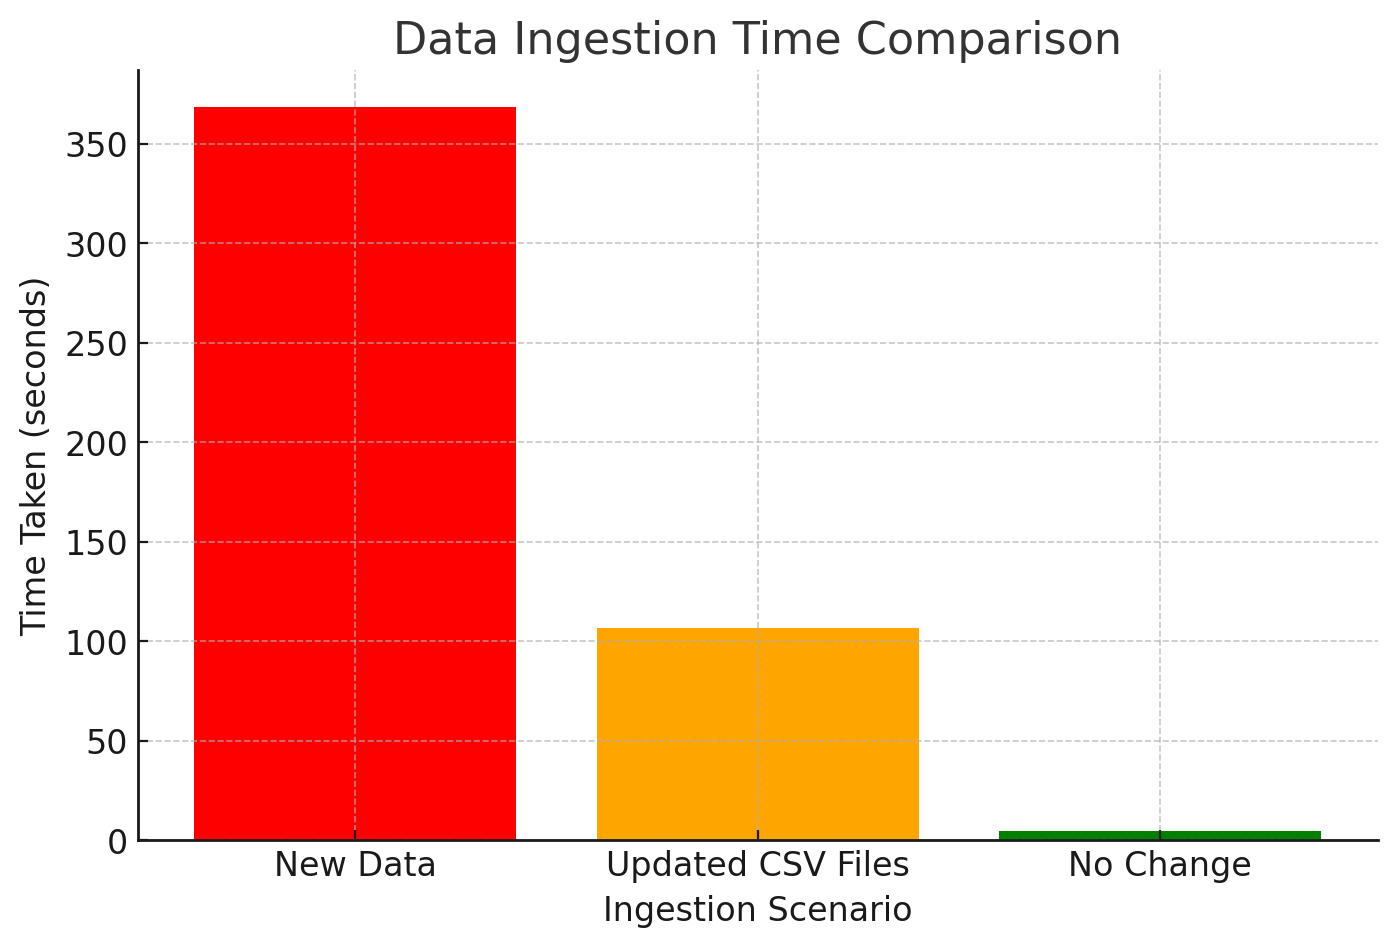
\includegraphics[width=7.2cm]{fig_ingestion_time.png}}
  \caption{Comparison of data ingestion time across cold-start, incremental-update, and no-change scenarios.}
  \label{fig:ingestion-time}
 \end{figure}

\section{\uppercase{Discussion}}
\label{sec:discussion}

On RQ1, under the current embedding model the adaptive pipeline does not beat BM25-only on any of the four automated similarity metrics -- it is statistically tied on BLEU and ROUGE-L, and significantly \emph{behind} on METEOR (confirmed under both a paired $t$-test and a matched Wilcoxon test) and, less conclusively, on BERTScore (significant under the paired $t$-test only; Section~\ref{subsec:novel-vs-baselines}) -- and remains statistically tied with full hybrid and with vector-only on all four. This supersedes an earlier revision's finding of a two-metric edge, which traced to a pre-retrain measurement that was never re-verified after the embedding model changed; we report the correction rather than the superseded number. What the pipeline adds is not a generation-quality win but capabilities none of the single-method baselines have at all: abstaining rather than guessing on the rare open-ended English query it cannot ground with adequate confidence (down to 0.5\% of queries after the exact-match and abstention-recalibration fixes below, from 10.5\% in an earlier revision); correctly answering multi-hop prerequisite-chain questions via graph traversal, a query shape no single retrieved chunk answers; and operating over a bilingual corpus with the same architecture and comparable retrieval-ablation results in both languages. On RQ2, direct ablation shows a mixed picture by component: fine-tuning the embeddings (Section~\ref{subsec:finetune}) and the unambiguous-match score guarantee (Section~\ref{subsec:unambiguous}) both produced a measured, positive effect; adaptive routing was directly tested, not merely inferred from the $\lambda$-sweep finding that motivated it, and found to be actively counterproductive on its own terms -- isolated to the entity-heavy queries where it can differ from a fixed baseline, it ties the baseline exactly under the deployed exact-match mechanism (Section~\ref{subsec:adaptive-isolated}), but with that mechanism's ranking ceiling removed as a deconfounding diagnostic, its RRF-fusion choice is significantly worse ($p<0.0001$ on Recall@1/3), showing the tie is a mechanism outside adaptive routing rescuing it, not evidence routing itself is a sound design choice; and the cross-encoder reranker produced a measured, significant \emph{negative} effect, which we confirmed is not simply an artifact of an undertrained reranker (fine-tuning it on the corpus's own hard negatives from the actual deployed retriever did not flip this result) nor of candidate-set noise from a wide reranking pool (restricting the pool to \texttt{final\_k}=5 candidates did not flip it either, Section~\ref{subsec:reranker-ablation}) -- on this corpus, the reranker's joint relevance judgments disagree with the fine-tuned embeddings' ranking under both explanations the literature offers for when reranking helps or hurts. On RQ3, the system performs comparably across languages on the retrieval ablation, and the two components built specifically for the code-mixed setting (query translation, BM25 normalization) show null effects on the main Banglish test set for a structural reason we then tested directly: a dedicated cross-lingual stress test (Section~\ref{subsec:crosslingual-stress}), built from EnglishQA content with no BanglishQA counterpart, shows query translation more than doubling top-5 retrieval accuracy (33.3\% to 77.8\%) in the scenario it was actually designed for -- confirming the null result was a test-set limitation, not evidence the technique is unhelpful.

We describe this paper's contribution deliberately as a validated engineering integration, not a novel retrieval algorithm: Reciprocal Rank Fusion \citep{cormack2009}, contrastive embedding fine-tuning \citep{henderson2017mnr}, cross-encoder reranking, graph-based multi-hop reasoning, confidence-gated abstention with a sufficiency override \citep{joren2024}, and confidence-ordered zig-zag context assembly \citep{liu2024lost,jin2024longcontext} are each individually established techniques. What we report as the contribution is that we combined them into one system for an under-studied bilingual academic-advising setting, ablated each component individually rather than only end-to-end, and report the resulting evidence -- including where components did not help -- rather than assume the combination is an improvement because each part is individually well-motivated. Where we come closest to a genuine unifying idea rather than a combination is Section~\ref{subsec:confidence-ordering}'s observation that abstention gating, context ordering, and (as future work) compression can all be driven by the same per-chunk confidence score computed once, and Section~\ref{subsec:crosslingual-sufficient-context}'s bilingual application of sufficient-context classification as a diagnostic for code-mixed retrieval specifically -- both modestly scoped, and reported as such.

\subsection{Limitations}

Several limitations qualify these findings, some resolved during this revision and some still open. First, we still have not produced a manual hallucination annotation; the automated LLM-judge faithfulness score (Section~\ref{subsec:faithfulness}) is a real, code-executed measurement but is a different instrument from human annotation against ground truth, uses a single automated judge with no second rater, and its lower point estimate for the adaptive pipeline relative to the baselines is only partially explained (Section~\ref{sec:discussion}). This is the one limitation on this list that cannot be resolved by more engineering effort alone -- it requires an actual second human rater, which is outside the scope of what this revision can produce. Second, the entity-heavy abstention threshold (Section~\ref{subsec:abstention}) was calibrated against only 18 naturally-occurring labeled examples; we grew this to 60 with database-verified synthetic examples (nonexistent vs.\ real course codes/faculty initials), tightening the 95\% CI on accuracy from (0.65, 0.99) to (0.861, 0.990) -- better, but the synthetic portion is template-generated rather than organic, which we disclose rather than blend in silently. Third, the open-ended abstention threshold's recall improved from 0.457 to 0.870 after recalibrating against the exact-match-fixed retriever (Section~\ref{subsec:unambiguous}); the sufficient-context override (Section~\ref{subsec:abstention}) still only ever makes the system \emph{less} likely to abstain, so it cannot itself compensate for missed detections, but the underlying gate is now substantially more sensitive than before. Fourth, the cross-lingual stress test identified as a gap in an earlier pass -- Banglish queries about content that exists only in EnglishQA -- has now been built and evaluated (Section~\ref{subsec:crosslingual-stress}); its main limitation is size (only 9 qualifying queries after deduplication), so its result is reported as suggestive rather than significance-tested. Fifth, the faithfulness sample sizes (40--50 per configuration) remain modest relative to the full 200-query English test set; we did apply paired bootstrap significance testing to them following \citet{dror2018hitchhiker}'s guidance that graded, potentially non-normally-distributed measures like faithfulness scores should use a non-parametric paired test rather than an assumed-normal paired $t$-test, but this was only possible in full among the four baseline configurations (confirmed to share the same 40 query\_ids); the adaptive-pipeline sample only overlaps the baselines' query\_ids on 17/40 rows, restricting that comparison to a smaller matched subset -- under which the adaptive pipeline's faithfulness gap versus every baseline is, in fact, \emph{not} statistically significant (all four comparisons $p\geq0.14$), a further (though small-$n$) piece of evidence that the raw descriptive gap in Table~\ref{tab:faithfulness} may not reflect a real effect. Sixth, this revision now runs on GPU (an NVIDIA RTX 3050 Ti, CUDA 12.1) rather than CPU-only, which resolves the previous hardware limitation for embedding fine-tuning and reranking, though BERTScore and generation-side wall-clock timings in Section~\ref{subsec:efficiency} predate this change and were not re-measured. Seventh, the independent NLI-based faithfulness cross-check (Section~\ref{subsec:nli-faithfulness}) itself has weak row-level agreement with the LLM judge (Pearson $r=0.089$); we treat its corroborating pattern at the aggregate level as suggestive evidence, not as a validated replacement metric, and note that building a genuinely reliable independent faithfulness signal remains open -- to that end we prepared, but have not yet completed, a 50-item disagreement-prioritized human annotation sample (the query\_ids where the LLM judge and the NLI check disagree most, plus a smaller agreement-anchor subsample), with blank rating columns for a human rater; this closes the machine-side half of a future human validation pass but the actual annotation, requiring a person, remains outside this revision's scope. Eighth, the FacultyAvailability coverage gap identified in an earlier pass has been closed (Section~\ref{subsec:faculty-coverage}), and we generalized the underlying lesson into a standing table-coverage audit (Section~\ref{subsec:patterns-refactor}) rather than leaving it as two one-off fixes; the audit currently finds no remaining zero-coverage table, though it can only ever prove a table has \emph{some} exercising query, not that its routing is correct in every case. Ninth, the LLM-based entity-normalization fallback (Section~\ref{subsec:abstention}) implemented to address the entity-heavy abstention gate's brittleness is not yet validated by its own ablation -- we confirmed the specific spacing/dash gap that motivated it with a direct, deterministic regex fix instead (verified live), and left the broader LLM-based fallback available but disabled by default, the same honest posture as query translation before it was properly tested. Tenth, the expanded cross-lingual stress test (27 queries, three LLM-generated Banglish phrasings each of the same 9 underlying facts) shows a more cautious picture than the original 9-query set: the direction still favors query translation (40.7\% vs.\ 55.6\% top-5 accuracy) but is not statistically significant on the discordant pairs (exact binomial $p=0.219$), and manual inspection found visible naturalness problems in a minority of the higher-temperature-generated variants, consistent with \citet{dogruoz2023representativeness}'s caution against treating LLM-generated code-switched text as equivalent to organically-collected data.

\subsection{Future Work}

The most direct remaining priority is a human hallucination annotation study on the current pipeline, with a second rater, to complement the automated faithfulness score. This is now better motivated than before: an independent, architecturally-separate NLI-based faithfulness cross-check (Section~\ref{subsec:nli-faithfulness}) does not reproduce the LLM-judge's finding that the adaptive pipeline is less faithful than the baselines, corroborating (without confirming) the hypothesis that this gap is a claim-decomposition artifact of self-judging rather than a genuine grounding regression -- a human rater is the direct way to settle this. A second priority is extending the cross-lingual stress test's small sample (Section~\ref{subsec:crosslingual-stress}) with more EnglishQA-only content as the corpus grows, since its current 9-query size limits it to a suggestive rather than a confirmatory result, even though its direction (query translation roughly doubling retrieval accuracy in the scenario it targets) is now demonstrated rather than merely hypothesized. A third is re-testing the sufficient-context override's net effect on precision/recall now that the underlying confidence gate is substantially more sensitive (Table~\ref{tab:abstention-calib}) than when the override was first validated.

This paper extended a hybrid BM25/dense RAG chatbot for academic advising into an adaptive pipeline combining domain-fine-tuned bilingual embeddings, per-query-type fusion routing, prerequisite-graph augmentation, and confidence-gated abstention with a sufficient-context override, and evaluated it on 200 English and 100 Banglish test queries with paired significance testing throughout, plus standard IR metrics (Recall@k, MRR, nDCG@10) and an independent NLI-based faithfulness cross-check. Under the current embedding model, the adaptive pipeline does not beat BM25-only on any of the four automated metrics (tied on BLEU/ROUGE-L, significantly behind on METEOR and, less conclusively, BERTScore) and remains statistically tied with full hybrid and vector-only on all four; a deconfounding diagnostic further shows adaptive routing's own fusion-method choice is significantly negative in isolation once the exact-match mechanism's ranking ceiling is removed, so the observed parity with the fixed baselines is borrowed entirely from that separate, independently-validated mechanism rather than being evidence that routing itself is beneficial. The system's real, defensible value is the abstention and multi-hop graph reasoning capabilities the baselines cannot perform at all, together with the entity-collision handling that drives the exact-match mechanism's own positive result, not a generation-quality edge over the single-method baselines. Embedding fine-tuning and an isolated unambiguous-match guarantee (extended in this revision to cover faculty lookups, not just course codes) each produced a measured positive effect; a cross-encoder reranker -- both a generic version and, after we caught and corrected a training/deployment mismatch, a properly fine-tuned one -- produced a measured negative effect in both cases; cross-lingual query translation showed a null effect on the main Banglish test set but a clear positive effect (33.3\% to 77.8\% top-5 accuracy) on a dedicated stress test built for the scenario it targets; and BM25-level code-mixed normalization remains a null result on the data tested. We describe the result as a validated system-level integration for an under-studied bilingual advising setting, disclose every limitation and every methodological pitfall (including our own) found along the way, and identify human hallucination annotation as the most direct remaining step toward a stronger generalization claim.

\section*{\uppercase{Ethical Statement}}

To protect student privacy, personal identifiers (names and student IDs) were removed from the dataset during ingestion, and community-sourced data was anonymized prior to analysis.

\section*{\uppercase{Acknowledgements}}

\begin{itemize}
  \item \textbf{Conflicts of Interest:} The authors have no conflicts of interest or competing interests to declare in the context of this paper.
  \item \textbf{Financial and other Support:} No funding was received for the work reported here.
  \item \textbf{Author Contributions:} The authors contributed equally.
  \item \textbf{Data Sharing:} A dataset was generated and analyzed during the current study, available at $<$url$>$.
  \item \textbf{AI Tools:} The paper used AI tools for text correction purposes only.
\end{itemize}

{\small
\begin{thebibliography}{99}

\bibitem[Adamopoulou and Moussiades(2021)]{adamopoulou2021} Adamopoulou, E. and Moussiades, L. (2021). Chatbots: History, technology, and applications. \textit{Machine Learning with Applications}, 2:100006.

\bibitem[Banerjee and Lavie(2005)]{banerjee2005} Banerjee, S. and Lavie, A. (2005). METEOR: An automatic metric for MT evaluation with improved correlation with human judgments. In \textit{Proceedings of ACL 2005}.

\bibitem[Brandtzaeg and F{\o}lstad(2017)]{brandtzaeg2017} Brandtzaeg, P. B. and F{\o}lstad, A. (2017). Why people use chatbots. In \textit{Internet Science (INSCI 2017)}, LNCS vol.\ 10673, pages 377--392. Springer, Cham.

\bibitem[Cormack et~al.(2009)]{cormack2009} Cormack, G. V., Clarke, C. L. A., and Buettcher, S. (2009). Reciprocal rank fusion outperforms Condorcet and individual rank learning methods. In \textit{Proceedings of the 32nd International ACM SIGIR Conference}, pages 758--759.

\bibitem[Athanasiou et~al.(2026)]{athanasiou2026semeval} Athanasiou, D., Lymperaiou, M., Filandrianos, G., Voulodimos, A., and Stamou, G. (2026). AILS-NTUA at SemEval-2026 Task 8: Evaluating multi-turn RAG conversations. In \textit{Proceedings of SemEval-2026}. arXiv:2603.10524.

\bibitem[Huang and Huang(2026)]{huang2026survey} Huang, Y. and Huang, J. X. (2026). A survey on retrieval-augmented text generation for large language models. \textit{ACM Computing Surveys}, 58(12), Article 300. arXiv:2404.10981.

\bibitem[Dror et~al.(2018)]{dror2018hitchhiker} Dror, R., Baumer, G., Shlomov, S., and Reichart, R. (2018). The hitchhiker's guide to testing statistical significance in natural language processing. In \textit{Proceedings of the 56th Annual Meeting of the Association for Computational Linguistics}, pages 1383--1392.

\bibitem[Do\u{g}ru\"oz et~al.(2023)]{dogruoz2023representativeness} Do\u{g}ru\"oz, A. S., Sitaram, S., and Yong, Z. X. (2023). Representativeness as a forgotten lesson for multilingual and code-switched data collection and preparation. In \textit{Findings of the Association for Computational Linguistics: EMNLP 2023}, pages 5751--5767. arXiv:2310.20470.

\bibitem[El-Ashmawi et~al.(2023)]{elashmawi2023} El-Ashmawi, W. H. et al. (2023). An interactive chatbot for college enquiry. \textit{Journal of Computing and Communication}, 2(1):20--28.

\bibitem[Es et~al.(2023)]{es2023ragas} Es, S., James, J., Espinosa-Anke, L., and Schockaert, S. (2023). RAGAS: Automated evaluation of retrieval augmented generation. \textit{arXiv preprint arXiv:2309.15217}.

\bibitem[Formica et~al.(2023)]{formica2023} Formica, A., Mele, I., and Taglino, F. (2023). A template-based approach for question answering over knowledge bases. \textit{Knowledge and Information Systems}, 65:453--479.

\bibitem[Henderson et~al.(2017)]{henderson2017mnr} Henderson, M., Al-Rfou, R., Strope, B., Sung, Y.-H., Lukacs, L., Guo, R., Kumar, S., Miklos, B., and Kurzweil, R. (2017). Efficient natural language response suggestion for smart reply. \textit{arXiv preprint arXiv:1705.00652}.

\bibitem[Goswami and Kurra(2025)]{halt2025} Goswami, S. and Kurra, S. (2025). HALT-RAG: A task-adaptable framework for hallucination detection with calibrated NLI ensembles and abstention. \textit{arXiv preprint arXiv:2509.07475}.

\bibitem[Laban et~al.(2022)]{summac2022} Laban, P., Schnabel, T., Bennett, P. N., and Hearst, M. A. (2022). SummaC: Re-visiting NLI-based models for inconsistency detection in summarization. \textit{Transactions of the Association for Computational Linguistics}, 10:163--177.

\bibitem[Hwang et~al.(2025)]{exit2025} Hwang, T., Cho, S., Jeong, S., Song, H., Han, S., and Park, J. C. (2025). EXIT: Context-aware extractive compression for enhancing retrieval-augmented generation. In \textit{Findings of the Association for Computational Linguistics: ACL 2025}. arXiv:2412.12559.

\bibitem[Jin et~al.(2024)]{jin2024longcontext} Jin, B., Yoon, J., Han, J., and Arık, S. Ö. (2024). Long-context LLMs meet RAG: Overcoming challenges for long inputs in RAG. \textit{arXiv preprint arXiv:2410.05983}.

\bibitem[Liu et~al.(2024)]{liu2024lost} Liu, N. F., Lin, K., Hewitt, J., Paranjape, A., Bevilacqua, M., Petroni, F., and Liang, P. (2024). Lost in the middle: How language models use long contexts. \textit{Transactions of the Association for Computational Linguistics}, 12:157--173.

\bibitem[Magomere et~al.(2025)]{magomere2025} Magomere, J., La Malfa, E., Tonneau, M., Kazemi, A., and Hale, S. (2025). When claims evolve: Evaluating and enhancing the robustness of embedding models against misinformation edits. In \textit{Findings of the Association for Computational Linguistics: ACL 2025}. arXiv:2503.03417.

\bibitem[Meghwani et~al.(2025)]{meghwani2025hardneg} Meghwani, H., Agarwal, A., Pattnayak, P., Patel, H. L., and Panda, S. (2025). Hard negative mining for domain-specific retrieval in enterprise systems. In \textit{Proceedings of the 63rd Annual Meeting of the Association for Computational Linguistics: Industry Track}. arXiv:2505.18366.

\bibitem[Huang et~al.(2023)]{huang2023} Huang, L., Yu, W., Ma, W., Zhong, W., Feng, Z., Wang, H., et al. (2023). A survey on hallucination in large language models: Principles, taxonomy, challenges, and open questions. \textit{ACM Transactions on Information Systems}.

\bibitem[Hwang and Chang(2021)]{hwang2021} Hwang, G.-J. and Chang, C.-Y. (2021). A review of opportunities and challenges of chatbots in education. \textit{Interactive Learning Environments}, 29(1):1--14.

\bibitem[Joren et~al.(2024)]{joren2024} Joren, H., Zhang, J., Ferng, C.-S., Juan, D.-C., Taly, A., and Rashtchian, C. (2024). Sufficient context: A new lens on retrieval augmented generation systems. \textit{arXiv preprint arXiv:2411.06037}.

\bibitem[Khanuja et~al.(2020)]{khanuja2020gluecos} Khanuja, S., Dandapat, S., Srinivasan, A., Sitaram, S., and Choudhury, M. (2020). GLUECoS: An evaluation benchmark for code-switched NLP. In \textit{Proceedings of ACL 2020}.

\bibitem[Lewis et~al.(2020)]{lewis2020} Lewis, P., Perez, E., Piktus, A., Petroni, F., Karpukhin, V., Goyal, N., et al. (2020). Retrieval-augmented generation for knowledge-intensive NLP tasks. \textit{Advances in Neural Information Processing Systems}, 33:9459--9474.

\bibitem[Lin(2004)]{lin2004} Lin, C.-Y. (2004). ROUGE: A package for automatic evaluation of summaries. \textit{Proceedings of ACL 2004}.

\bibitem[Nguyen et~al.(2023)]{nguyen2023lilo} Nguyen, H., Lopez, J., Homer, B., Ali, A., and Ahn, J. (2023). Reminders, reflections, and relationships: Insights from the design of a chatbot for college advising. \textit{Information and Learning Sciences}, 124(3/4):128--146.

\bibitem[Papineni et~al.(2002)]{papineni2002} Papineni, K., Roukos, S., Ward, T., and Zhu, W.-J. (2002). BLEU: A method for automatic evaluation of machine translation. In \textit{Proceedings of ACL 2002}.

\bibitem[Reimers and Gurevych(2019)]{reimers2019sbert} Reimers, N. and Gurevych, I. (2019). Sentence-BERT: Sentence embeddings using Siamese BERT-networks. In \textit{Proceedings of EMNLP-IJCNLP 2019}.

\bibitem[Rahman et~al.(2025)]{rahman2025mentorship} Rahman, M., Abedin, M., Abir, M. Z., Ansari, M. F. I., Reza, A., Sadeque, F. Y., and Farhan, N. (2025). Transforming mentorship: An AI powered chatbot approach to university guidance. \textit{arXiv preprint arXiv:2511.04172}.

\bibitem[Zeng et~al.(2026)]{zeng2026codeswitching} Zeng, Q., Lu, Y., Zhou, Z., Qi, H., Yu, P., Zhao, F., Yanaka, H., Xuan, W., and Yokoya, N. (2026). Code-switching information retrieval: Benchmarks, analysis, and the limits of current retrievers. In \textit{Findings of the Association for Computational Linguistics: ACL 2026}. arXiv:2604.17632.

\bibitem[Kruk et~al.(2025)]{kruk2025banglassist} Kruk, F., Herath, S., and Choudhury, P. (2025). BanglAssist: A Bengali-English generative AI chatbot for code-switching and dialect-handling in customer service. In \textit{Extended Abstracts of the CHI Conference on Human Factors in Computing Systems (CHI EA '25)}. arXiv:2503.22283.

\bibitem[Xiang et~al.(2025)]{xiang2025graphs} Xiang, Z., Wu, C., Zhang, Q., Chen, S., Hong, Z., Huang, X., and Su, J. (2025). When to use graphs in RAG: A comprehensive analysis for graph retrieval-augmented generation. \textit{arXiv preprint arXiv:2506.05690}.

\bibitem[Jacob et~al.(2024)]{jacob2024drowning} Jacob, M., Lindgren, E., Zaharia, M., Carbin, M., Khattab, O., and Drozdov, A. (2024). Drowning in documents: Consequences of scaling reranker inference. \textit{ReNeuIR 2025 Workshop at SIGIR 2025}. arXiv:2411.11767.

\bibitem[Chen et~al.(2025)]{chen2025scirerankbench} Chen, H., Long, Q., Xiao, M., Luo, X., Ju, W., Wang, C., Wang, X., Zhou, Y., and Zhu, H. (2025). SciRerankBench: Benchmarking rerankers towards scientific retrieval-augmented generated LLMs. \textit{arXiv preprint arXiv:2508.08742}.

\bibitem[Panickssery et~al.(2024)]{panickssery2024selfpref} Panickssery, A., Bowman, S. R., and Feng, S. (2024). LLM evaluators recognize and favor their own generations. \textit{arXiv preprint arXiv:2404.13076}.

\bibitem[Robertson and Zaragoza(2009)]{robertson2009} Robertson, S. and Zaragoza, H. (2009). The probabilistic relevance framework: BM25 and beyond. \textit{Foundations and Trends in Information Retrieval}.

\bibitem[Sawarkar et~al.(2024)]{sawarkar2024} Sawarkar, K., Mangal, A., and Solanki, S. R. (2024). Blended RAG: Improving RAG (retriever-augmented generation) accuracy with semantic search and hybrid query-based retrievers. \textit{arXiv preprint arXiv:2404.07220}.

\bibitem[Shawar and Atwell(2007)]{shawar2007} Shawar, B. A. and Atwell, E. (2007). Chatbots: Are they really useful? \textit{LDV Forum}, 22(1):29--49.

\bibitem[Swacha and Gracel(2025)]{swacha2025} Swacha, J. and Gracel, M. (2025). Retrieval-augmented generation (RAG) chatbots for education: A survey of applications. \textit{Applied Sciences}, 15(8):4234.

\bibitem[Varshney et~al.(2023)]{varshney2023} Varshney, N., Yao, W., Zhang, H., Chen, J., and Yu, D. (2023). A stitch in time saves nine: Detecting and mitigating hallucinations of LLMs by validating low-confidence generation. \textit{arXiv preprint arXiv:2307.03987}.

\bibitem[Zhang et~al.(2019)]{zhang2019} Zhang, T., Kishore, V., Wu, F., Weinberger, K. Q., and Artzi, Y. (2019). BERTScore: Evaluating text generation with BERT. In \textit{Proceedings of ICLR 2019}.

\end{thebibliography}
}

\end{document}
